%
% Unless otherwise indicated, the copyright in this material is 
% owned by Joerg Evermann. This material is licensed to you under the 
% Creative Commons by-attribution non-commercial license (CC BY-NC 4.0)}
%
\section*{Learning Goals}

After reading this chapter, you should be able to:
\begin{itemize}
   \item Explain the purpose and illustrate different methods for data augmentation for neural network training.
   \item Describe transfer learning and fine-tuning for predictive models.
   \item Explain attention, self-attention, and multi-headed attention in deep-learning architectures.
   \item Define a transformer architecture with its components of encoder and decoder.
   \item Describe popular language models such as BERT and GPT models and their differences.
   \item Explain the principles and applications of auto-encoders and variational auto-encoders and the differences between them.
   \item Describe the principles and architecture of generative adversarial networks.
\end{itemize}

\section*{Sources and Further Reading}

\begin{resourcebox}
Kevin P. Murphy: \emph{Probabilistic Machine Learning -- An Introduction}. MIT Press 2022. \\

\small\url{https://probml.github.io/pml-book/book1.html}\normalsize \\

Chapters 15, 19, 20
\end{resourcebox}

The book by Murphy is freely available and provides three chapters on neural networks, one for structured data, one for images, and one for sequences. It provides significant depth on convolutional and recurrent network architectures, fitting the models, and problems the data analyst may encounter. 

\begin{resourcebox}
Foster, D: \emph{Generative Deep Learning}, 2nd edition. O'Reilly Media 2022. \\

\vspace{0.5\baselineskip}

Chapters 3, 4, 9, 10
\end{resourcebox}

The book by Foster is more applied than the book by Murphy. It focuses on generative neural-network models for image generation, text generation, music generation, etc. While some of the foundational details are provided, the book focuses on implementation of the models in Python and offers many code examples with illustrations and explanations.

\begin{resourcebox}
Zhang, A., Lipton, Z.C., Li, M. and Smola, A.J.: \emph{Dive into Deep Learning (D2L)}. Cambridge University Press. 2023. \url{https://d2l.ai/} \\
\end{resourcebox}

The book by Zhang et al. is an open-source, ''living'' book that can also be found on Github and its website. It focuses on deep learning models only and provides a thorough treatment of the material with Python examples for a variety of deep learning frameworks, including PyTorch and TensorFlow. It is light on the math, but does explain the concepts well with diagrams and a few formulas. It focuses on the implementation of the ideas in actual code. 


\section{Data Augmentation}

Data augmentation\index{Data augmentation} is used to create additional synthetic training data, typically for use with deep neural network classification models. Data augmentation serves a variety of purposes:

\begin{enumerate}
\item One purpose is to \emph{increase the size} of the training data. This is not done by merely replicating existing input data, as the model would learn little from duplicated data and may even learn a wrong distribution of classes for classification problems. Instead, data augmentation is used to generate synthetic data that is similar to existing data but not identical. For example, image data may be rotated, translated, cropped etc. 

\item A second purpose of data augmentation is to serve as a \emph{regularization method} to guard against model overfitting. Used in this way, it provides more variation to the training data that prevents a model to learn the training data exactly. For example, consider replacing words with their synonyms in the training data for a text classification task. 

\item A third purpose is to ensure \emph{realistic training data}. The available training data may be too ''perfect'' in the sense that realistic noise is missing. In such cases, synthetic training data could be created by adding noise or other realistic variations to training data instances so that the model performs well when using real inputs that are often noisy.

\item A fourth purpose is  \emph{class balancing}. Consider a classifier trained on a data set with a strong majority class, for example a data set where 90\% of instances are of majority class $C$. A classifier might then exploit this fact at the expense of being able to identify minority classes. Class balancing creates additional synthetic samples to ensure minority classes are adequately represented in the training data and to prevent the model from capitalizing on a majority class.
\end{enumerate}

With these purposes in mind, data augmentation uses a variety of different methods. First, it creates additional data that is similar to existing training data instances. This is useful for increasing the sample size of training data, or when using data augmentation as a regularization method. Second, it can be used to create additional variations not already present in the training data. This is useful when data augmentation is used to ensure the training data is realistic and reflects what a model might be served as input at inference or prediction time. A third method is to introduce random noise to the training data. This is useful when the existing data is too clean and realistic input at inference or prediction time is expected to be noisy. Finally, data augmentation may use synthetic oversampling of minority classes in order to balance the class distribution in the training data set. 

\begin{figure}
\begin{center}
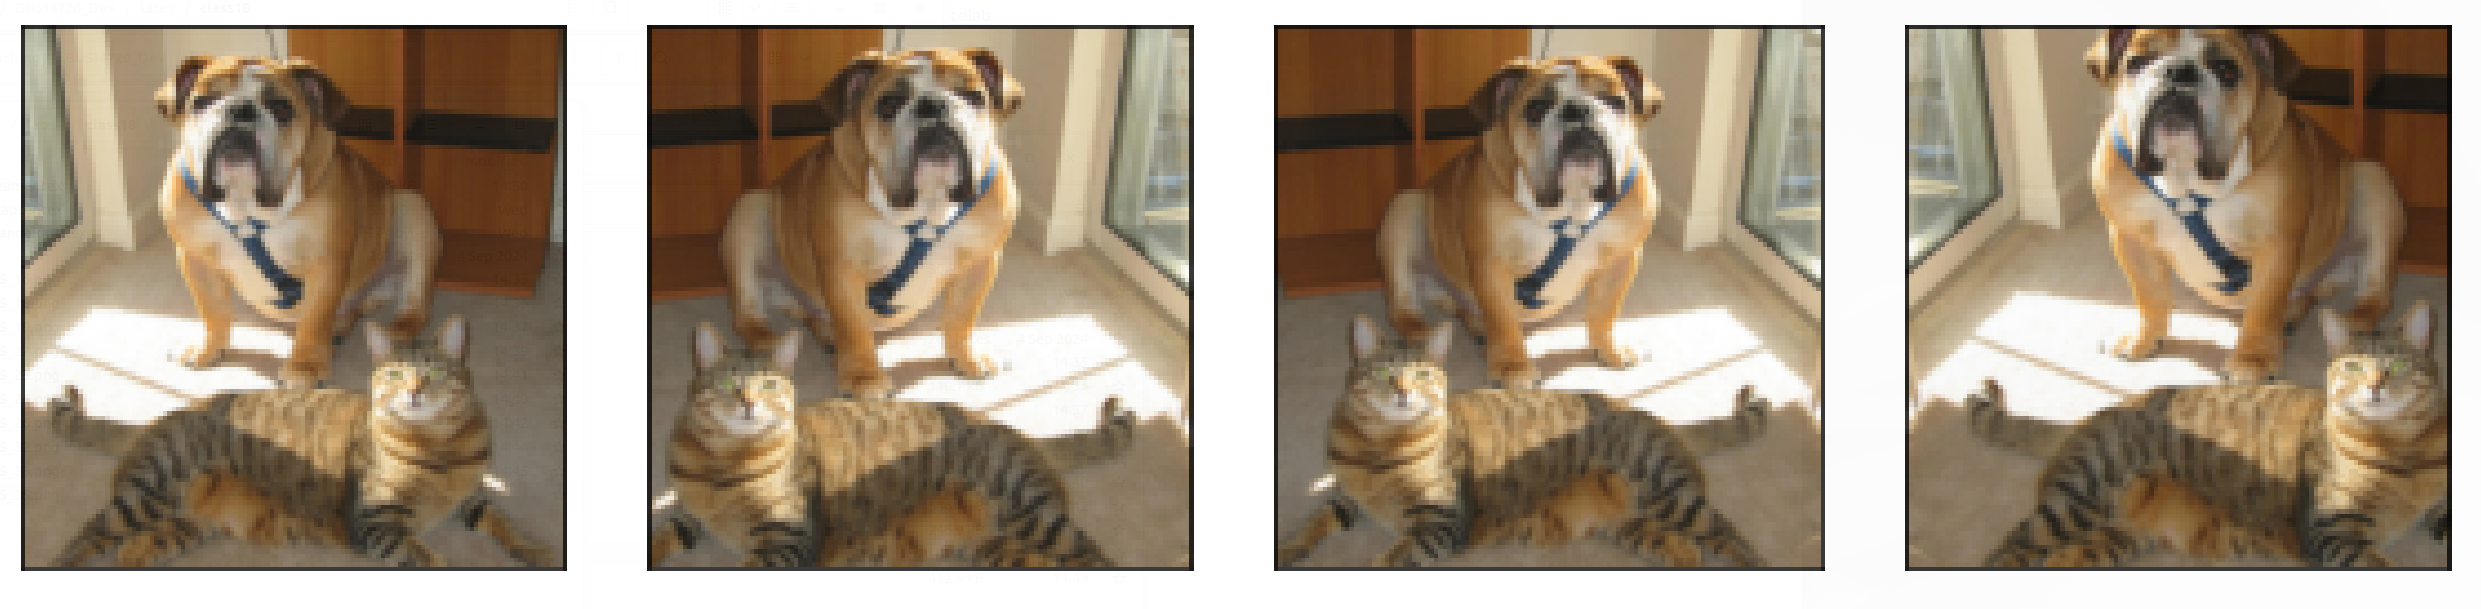
\includegraphics[width=\textwidth]{murphy_19_01.png} \\

\scriptsize Source: Murphy Fig. 19.1
\end{center}
\caption{Examples of data augmentation for image data}
\label{fig:murphy_19_1}
\end{figure}

Data augmentation for visual data is done using geometric transformations of existing images, such as rotating, flipping/mirroring, cropping, or translating the image, as illustrated in Figure~\ref{fig:murphy_19_1}. This creates additional data that is similar yet sufficiently different to serve as regularization, i.e. to prevent a trained model from simply learning or remembering the training data and forcing it to generalize or abstract to realistic variants of the training images. These transformations also create more realistic images than ideal training data images. Similarly, colour space transformations such as changes to brightness, contrast, and saturation can create additional data. Noise can be injected by randomly switching pixels in images to black or some random colour. Finally, kernel filters can be used to smooth or blur images or parts of images.  

Data augmentation for textual data uses techniques such as character, word, or sentence shuffling within the text. For example, with a small probability characters within words are swapped, or words within sentences are swapped, or sentences within a text are swapped. This too creates additional data that is similar to the training data yet different enough to serve as a regularization method. Another frequently used technique is the substitution of words with their synonyms or similar terms. Words may be deleted from a sentence at random (or characters from words). A technique unique to text data is the insertion of noise at the embedding level. Once an input word has been converted to a numeric vector, the values of this vector may be randomly ''jiggled'', that is, changed slightly, before they are provided as input for training a model. Also unique to text is the idea of forward--backward translation. For example, a sentence in English may be translated to Inuktitut, and then that sentence is translated back to English. This often leads to sentences with the same or similar meaning but using different words or sentence structure. 

\begin{figure}
\centering
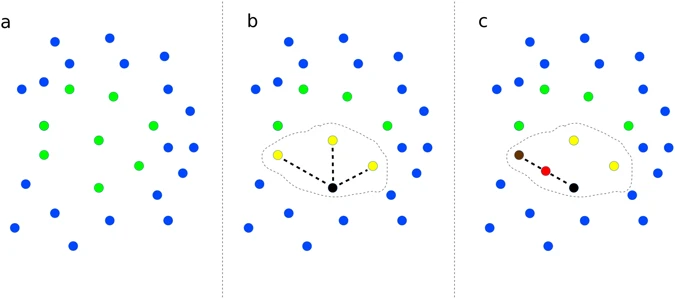
\includegraphics[width=\textwidth]{smote.png} 

\tiny Source: Schubach, M., Re, M., Robinson, P.N. et al. Imbalance-Aware Machine Learning for Predicting Rare and Common Disease-Associated Non-Coding Variants. Sci Rep 7, 2959 (2017). \url{https://doi.org/10.1038/s41598-017-03011-5} (CC-BY-4.0)
\normalsize
\caption{SMOTE principles}
\label{fig:smote}
\end{figure}

Data augmentation for tabular data, that is, numeric data uses techniques such as SMOTE\index{Synthetic Minority Oversampling Technique}\index{SMOTE|see{Synthetic Minority Oversampling Technique}} and SMOTE-NC. As its name implies, SMOTE (''synthetic minority oversampling technique'') is designed for class balancing, that is to create additional instances of a minority class in classification model training. Originally developed for The idea of SMOTE is simple and intuitive. Consider Figure~\ref{fig:smote}. The left panel shows observations for two classes in a two-dimensional continuous feature space. When generating an additional observation for the green class, SMOTE first determines the $k$ nearest neighbours of one observation for some value of $k$ (center panel in Figure~\ref{fig:smote}). Then, one of the neighbours is chosen at random, and an additional observation is created at some random distance between the focal observation and the chosen neighbour (right panel in Figure~\ref{fig:smote}). SMOTE-NC is the generalization of SMOTE to categorical features.

A variational auto-encoder is described in Section~\ref{sec:vae} below. The main idea is that input data is encoded into feature space that is a probability distribution, typically Gaussian or normal, characterized by a mean vector and a covariance matrix. To generate a new observation, one simply samples from a Gaussian and decodes the result. VAEs are popular with image data, underlying many popular generative AI image generators, but can also be used with tabular data for data augmentation purposes. In a broad sense, this could be seen as analogous to text data augmentation by ''jiggling'' the embedding (except text embeddings are not characterized by a probability distribution). 

\section{Transfer Learning}

The idea behind transfer learning\index{Transfer learning} is to transfer learned models to related domains. For example, consider a deep convolutional neural network that has been trained to classify cars. Using this CNN to classify trucks, which are assumed to be similar to cars, is an instance of transfer learning. The main assumptions are that the input data remains similar, e.g. images in this example of cars and trucks, and of a related domain. It would not be sensible to expect a CNN trained on birds to be useful for classifying cars. In other words, the features learned by the convolutional portion of a ConvNet classifier (e.g. edges, circles, boxes, wheels, etc. in this example) need to be useful features also for classification in the related domain. The main benefit of transfer learning is the reduction of expensive training effort and training data collection. 

A typical use case for transfer learning is to adapt models to data-poor tasks that are similar to other tasks for which a great amount of training data may be available. For example, classifying endangered bird species is difficult because of the small amount of available image data of endangered birds. However, with the assumption that ''bird features'' learned by a CNN for all birds are also useful for classifying endangered birds, a pre-trained CNN can be adapted. 

A second use case is to provide pre-trained models for classification. For example, an organization may train a predictive model on vehicle images, and provide or sell this pre-trained model to other organizations that wish to recognize similar objects in their input data. Pre-trained models are also feasible for text data, where a model could be trained on a general corpus and then be adapted by an organization for their specific input data. 

Transfer learning consists of two phases. In the first \emph{pre-training}\index{Pre-training (in transfer learning)} phase, a model is trained on a large source data set. In the second \emph{fine-tuning}\index{Fine-tuning (in transfer learning)} phase, the pre-trained model is further trained on a smaller target data set. A typical fine-tuning approach for classification models is to retain the feature extraction portion of the model and swap in a new classification ''head'' or classification portion, as shown in Figure~\ref{fig:murphy_19_02}. In this example, the model on the left shows the original model whose layers have been pre-trained on some some domain. For example, layers $1$ through $i-1$ may be the convolutional layers of a ConvNet while the output layer is a dense softmax classification layer. Transfer learning then consists of copying the model retaining pre-trained weights and biases, and swapping in a new, untrained classification ''head'' whose weights and biases are initialized randomly (in practice, multiple dense layers may be used after feature extraction layers and all or only some of them could be swapped out). At this point the new model can recognize or extract features based on the pre-trained layers but is not yet able to accurately classify observations based on their features. The fine-tuning phase then trains the new output layer from scratch, while making no or only small changes to the parameters in the pre-trained layers, that is, either fixing/freezing the parameter values or using a very small learning rate. The motivation is not to disturb the pre-trained weights to the point where the feature extraction is no longer sufficient for classification. 

\begin{figure}
\begin{center}
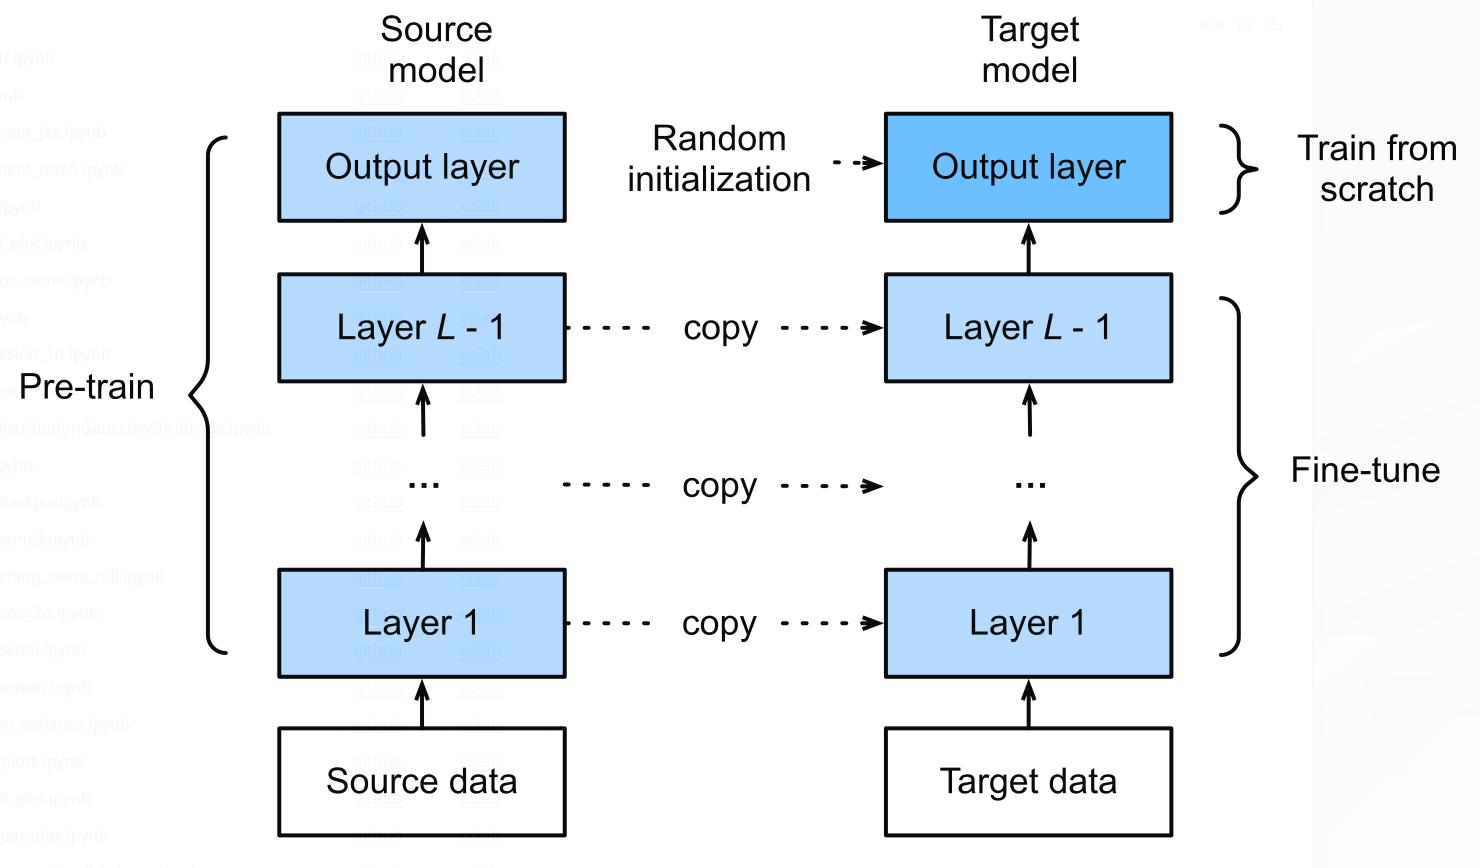
\includegraphics[width=0.8\textwidth]{murphy_19_02.png} \\
\scriptsize Source: Murphy Fig 19.2 \normalsize
\end{center}
\caption{Transfer learning for a classification model}
\label{fig:murphy_19_02}
\end{figure}

One problem with pre-training is that it may be slow for large models, that is models with many parameters in the pre-trained layers, all of which are updated with a small learning rate. Another problem is that the fine-tuned values may diverge too far from prior values, making the feature extraction layers useless. \emph{Adapters}\index{Adapter (in transfer learning)} address this problem. Adapters are small neural networks, typically a single or a few dense layers that are inserted between the feature extraction layers of a pre-trained network. The pre-trained layer parameter values are then fixed and the adapters are trained from scratch. This ensures that parameter values do not diverge from their pre-trained values and reduces the number of parameters to be trained, limited to the parameters in the adapters. 

Figure~\ref{fig:murphy_19_03} illustrates this idea in a transformer architecture (a) and a ResNet architecture (b). The adapter in panel (a) consists of a dense layer that reduces the dimensionality, then applies a non-linear activation function, followed by another dense layer that increases the dimensionality to that of the original input. If the input and output dimensionality is $d$ and the reduced dimensionality (also called ''bottleneck'' dimensionality) is $k$, there are $2 d k$ parameters in the adapter. Two adapters are inserted in each transformer layer.

The ''skip-connection'' or bypass connection allows the adapter parameters to be initialized to zero and therefore initially have no effect. This ensures that training of the classification layer begins with unchanged pre-trained parameters and features. 

In panel (b) of Figure~\ref{fig:murphy_19_03} $\alpha$ indicates a $1 \times 1$ convolutional layer and BN is a batch-normalization layer. The panel indicates two options for inserting this adapter, either in sequence (left) or in parallel (right). In this architecture also, initializing the convolution kernel to $0$ means the adapter initially has no effect. 

\begin{figure}
\centering
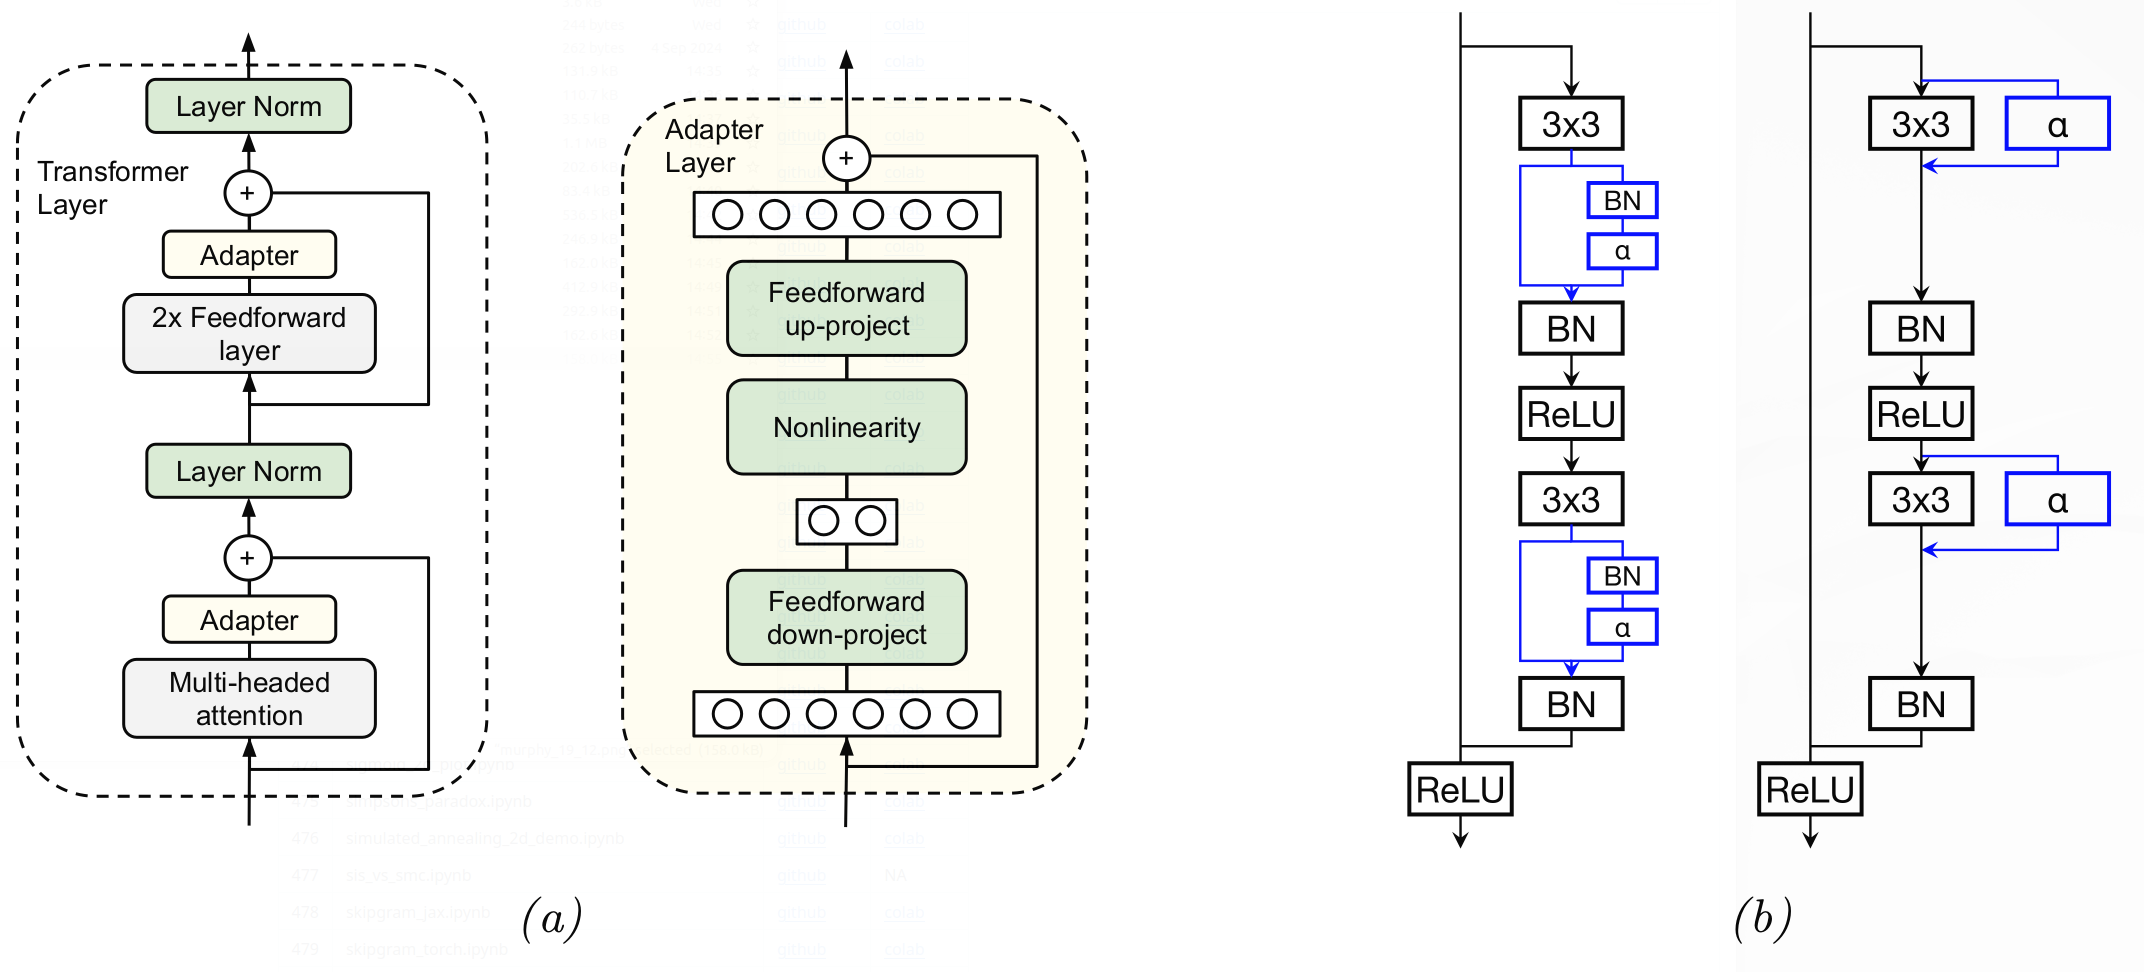
\includegraphics[width=\textwidth]{murphy_19_03.png} \\
\scriptsize Source: Murphy Fig. 19.3 \normalsize
\caption{Adapters in a transformer (a) and a ResNet (b)}
\label{fig:murphy_19_03}
\end{figure}

\FloatBarrier

\section{Data Augmentation and Transfer Learning in Python}

The example in this section illustrates both data augmentation and transfer learning in the context of image classification. The example uses a data set provided as part of the TensorFlow/Keras packages and a pre-trained image classification models, also part of the TensorFlow/Keras packages for Python. 

\begin{resourcebox}
Adapted from: 

\small\url{https://keras.io/guides/transfer_learning/}\normalsize \\

Implementation available on the following GitHub repo:

\small\url{https://github.com/jevermann/busi4720-ai}\normalsize \\

The project can be cloned from this URL:

\small\url{https://github.com/jevermann/busi4720-ai.git}\normalsize
\end{resourcebox}

First, the data set is loaded. This is a data set of cat and dog images, with two classes. The data set contains only a training data portion, which is split into training and test data as the data are loaded:

\begin{pythoncode}
import keras
from keras import layers
import tensorflow_datasets as tfds

# Load a Tensorflow example image data set
train_ds, test_ds = tfds.load(
    "cats_vs_dogs",
    split=["train[:75%]", "train[75%:100%]"],
    as_supervised=True)
\end{pythoncode}

The following code block resizes all images to the same size of $150 \times 150$ pixels using a Keras resizing layer.
\begin{pythoncode}
# Create Resizing layer
resize_fn = keras.layers.Resizing(150, 150)

# Apply resizing layer to data sets
train_ds = train_ds.map(lambda x, y: (resize_fn(x), y))
test_ds = test_ds.map(lambda x, y: (resize_fn(x), y))
\end{pythoncode}

Keras provides a number of image pre-processing layers that can be used for data augmentation. The following example uses all but the crop layer to illustrate the variety of transformations available. In practice, not all may be used, and not all may be applied to each image. The code block creates a sequential model consisting of a sequence of random transformation layers and then applies this model to the training data:

\begin{pythoncode}
# Define a sequential model of random transformation layers
augmentation = keras.models.Sequential([
    layers.RandomFlip("horizontal"),
    layers.RandomTranslation(.2, .2, fill_mode="reflect"),
    layers.RandomRotation(0.2, fill_mode="reflect"),
    layers.RandomZoom(.2, .2, fill_mode="reflect"),
    layers.RandomContrast(0.2),
    layers.RandomBrightness(0.2)])

# Apply augmentation model to training data
train_ds = train_ds.map(lambda x, y: (augmentation(x), y))
\end{pythoncode}

\begin{infobox}
\begin{itemize}
   \item This example applies all layers to all training images; consider applying single transformations to an image or random combinations of transformations
   \item This example replaces the data set with the transformed images; consider adding the transformed images to the data set
\end{itemize}
\end{infobox}

The following Python code loads an image classification model as a base model and a set of pre-trained weights for this model. Importantly, it does \emph{not} load the classification layer (\small\texttt{include\_top = False}\normalsize). The original data set the model was trained on has 1000 classes, but in this example application, the classification is only between cats and dogs, that is, two classes.
 
\begin{pythoncode}
base_model = keras.applications.Xception(
    weights="imagenet",
    input_shape=(150, 150, 3),
    include_top=False)
\end{pythoncode}

The base model's parameters are frozen/fixed by making the base model not trainable:
\begin{pythoncode}
base_model.trainable = False
\end{pythoncode}

To use the cats--dogs data set as input, the image data must be rescaled from $[0, 255]$ to $[-1, +1]$ using a Keras rescaling layer applied to the inputs:
\begin{pythoncode}
# Create new input model
inputs = keras.Input(shape=(150, 150, 3))
# Pre-trained Xception weights requires input scaling
# from [0, 255] to [-1., +1.]
scale_layer = keras.layers.Rescaling(scale=1/127.5, offset=-1)
x = scale_layer(inputs)
\end{pythoncode}

The scaled inputs can then be used by the base model. Training is set to \texttt{False} for the base model. A subsequent classification model is added, consisting of pooling, dropout, and dense layers. The complete model's summary confirms that not all parameters are trainable.
\begin{pythoncode}
x = base_model(x, training=False)
x = keras.layers.GlobalAveragePooling2D()(x)
x = keras.layers.Dropout(0.2)(x)
outputs = keras.layers.Dense(1)(x)

# Complete model has inputs and outputs
model = keras.Model(inputs, outputs)
# Not all parameters are trainable
model.summary(show_trainable=True)
\end{pythoncode}

The complete model (training only the classification layers) is compiled with the default learning rate for the chosen optimizer and then fitted in 2 epochs in the following Python code block. 

\begin{infobox}Only a few epochs are needed as the CNN portion of the model that serves as feature extractor is pre-trained and the classification portion of the model contains only relatively few trainable parameters.\end{infobox}


\begin{pythoncode}
model.compile(
    optimizer=keras.optimizers.Adam(),
    loss=keras.losses.BinaryCrossentropy(from_logits=True),
    metrics=[keras.metrics.BinaryAccuracy()],
)
model.fit(train_ds.batch(64), epochs=2, 
          validation_data=test_ds.batch(64))
\end{pythoncode}

As an alternative, the following Python code block shows how the base model parameters may also be fine-tuned using a very small learning rate for the optimizer. For this, the base model's parameters are made trainable and the model is compiled and fitted as usual:
\begin{pythoncode}
# Make all parameters trainable
base_model.trainable = True
# Now all parameters are trainable
model.summary(show_trainable=True)

# Very small learning rate
model.compile(
    optimizer=keras.optimizers.Adam(1e-5),
    loss=keras.losses.BinaryCrossentropy(from_logits=True),
    metrics=[keras.metrics.BinaryAccuracy()],
)
model.fit(train_ds.batch(64), epochs=2, 
          validation_data=test_ds.batch(64))
\end{pythoncode}

\section{Attention}

The concept of attention\index{Attention} is motivated from sequence-to-sequence models used for language translation. In ''traditional'' neural networks, all input features are weighted, then summed, and then passed through a non-linear activation function. In contrast, the attention mechanism allows a neural network to choose which input value $V$ to pay attention to (that is, which input to provide as output) based on the similarity of the input's key $K$ to some query vector $K$. 

\begin{figure}
\centering
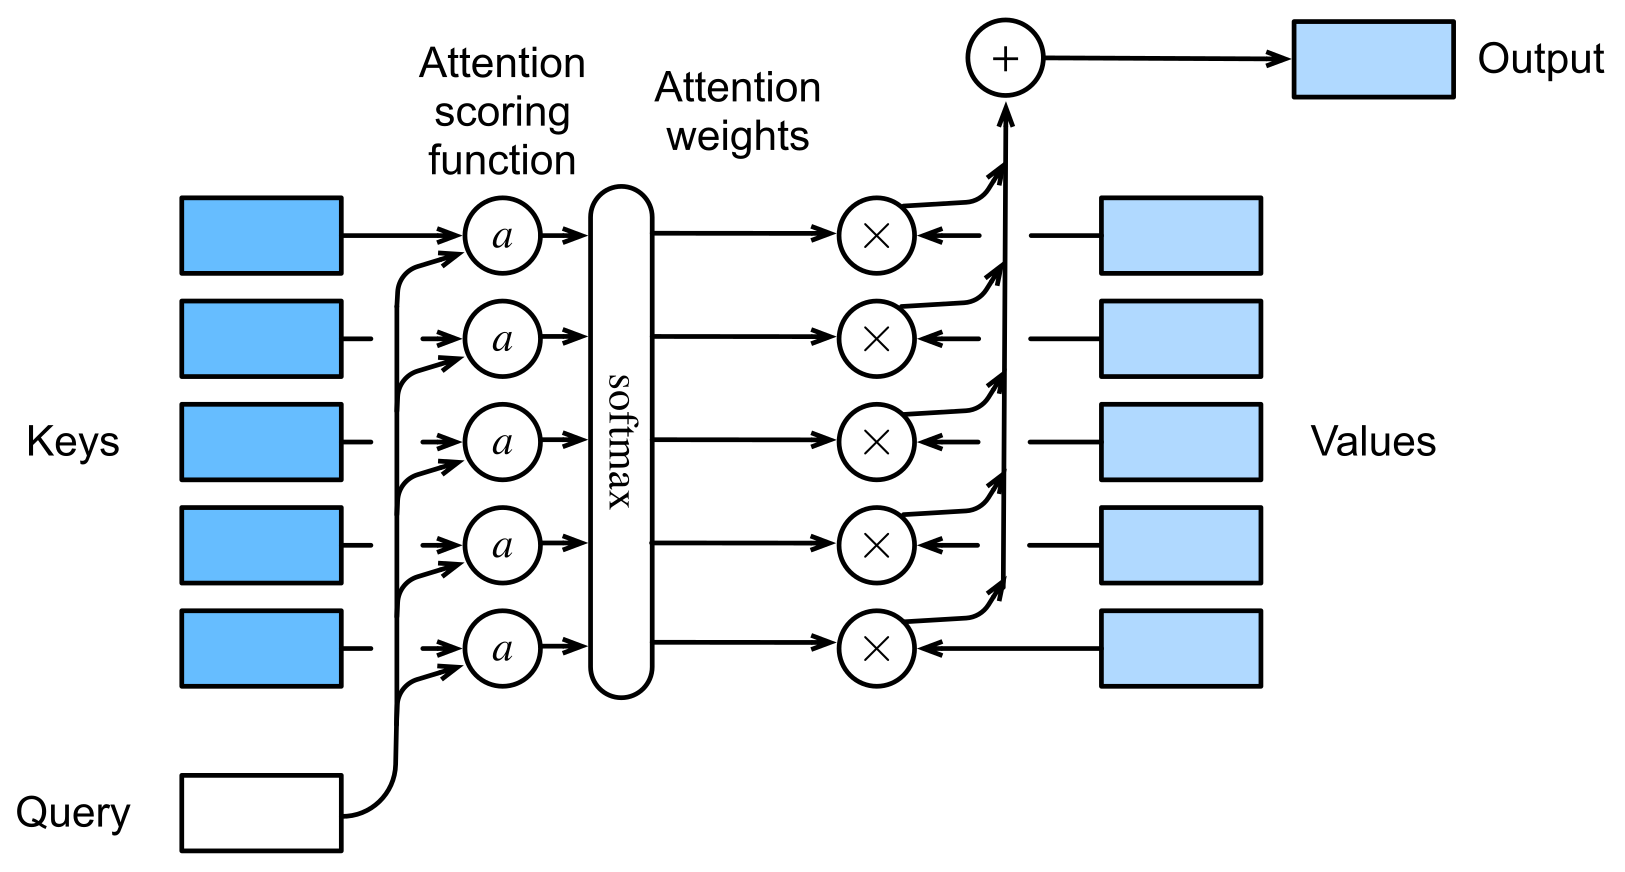
\includegraphics[width=.8\textwidth]{murphy_15_16.png} \\

\scriptsize Source: Murphy, Fig. 15.16 \normalsize
\caption{Attention in neural networks}
\label{fig:murphy_15_16}
\end{figure}

Consider the illustration in Figure~\ref{fig:murphy_15_16}. Each of the $m$ value vectors in $V$ has an associated key vector in $K$. Additionally, $Q$ is a ''query vector'' of the same dimensionality as each vector in $K$. The \emph{attention score}\index{Attention!score} function $a$ is a function that determines how similar each key is to the query vector $Q$. A softmax layer transforms the attention scores to \emph{attention weights}\index{Attention!weight} in the interval $[0, 1]$. Each of the $m$ values in $V$ is then multiplied with its attention weight and the products are summed to yield the output.  

Mathematically, attention is often defined as follows:

\begin{align*}
\operatorname{Attn}(Q, K, V) = \operatorname{softmax}\left(\frac{Q K^T}{\sqrt{d_k}} \right) V
\end{align*}

Here, the attention scoring function $a$ is the dot product of keys and query vector, scaled by the dimensionality of the keys. Consequently, this is called the ''scaled dot-product attention'' but other attention functions are possible and have been used in some applications. 

\begin{align*}
a(Q, K) = \frac{Q K^T}{\sqrt{d_k}}
\end{align*}

where $K$ is a matrix of $m$ key vectors, each of dimensionality $d_k$ and $V$ is a matrix of $m$ corresponding value vectors. 

\begin{figure}
\centering

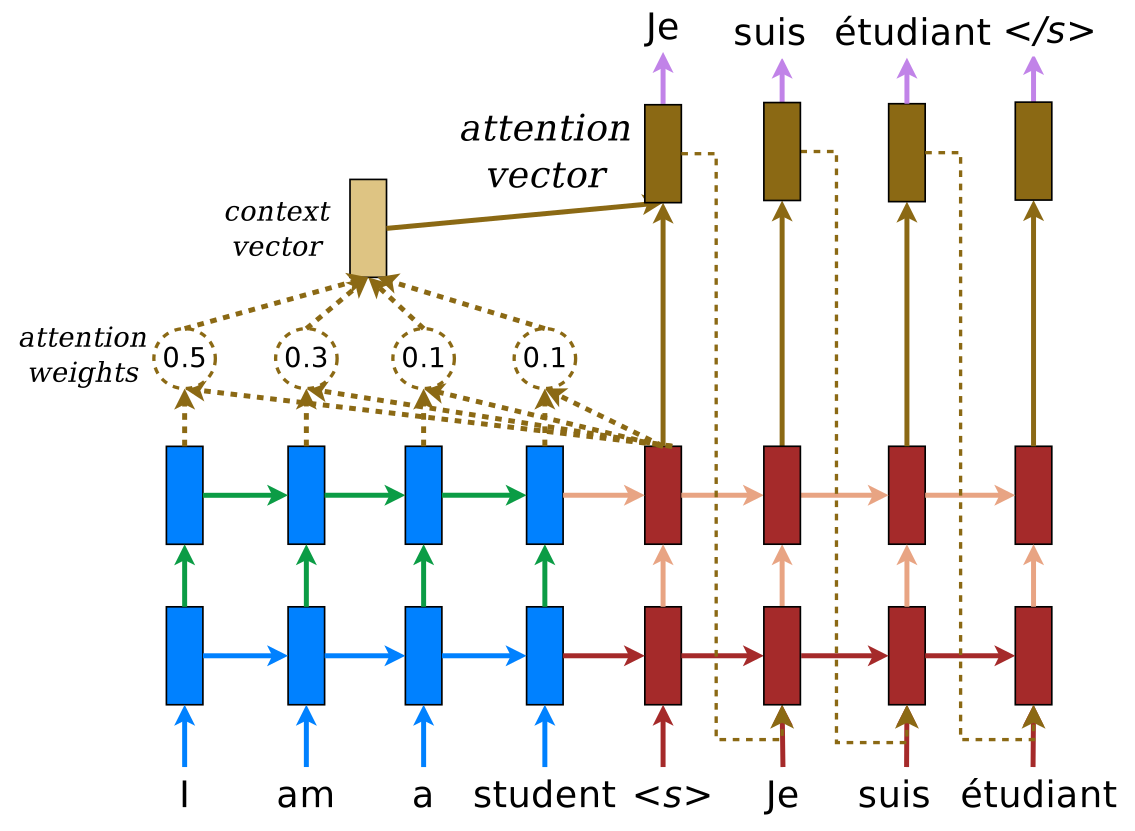
\includegraphics[width=.8\textwidth]{murphy_15_18.png} \\

\scriptsize Source: Murphy, Fig. 15.18 \normalsize
\caption{Attention in sequence-to-sequence model}
\label{fig:murphy_15_18}
\end{figure}

A example of the use of attention is the sequence-to-sequence model in Figure~\ref{fig:murphy_15_16} consisting of an encoder (blue cells) and a decoder (red cells). These could be some recurrent cells, such as LSTM or GRU cells. In ''traditional'' sequence-to-sequence models presented in a previous chapter, the context vector used for the decoder is static and is usually the hidden state of the final step $T$ of the encoder. That is:

\begin{align*}
c = h^e_T
\end{align*}

This is inefficient for a number of reasons. First, the decoder can only begin decoding after the final input token is processed. Also, for long input sequences, the encoding into a however sized hidden state vector is bound to lose details that cannot be recovered by the decoder. Finally, the decoder does not have access to the input words, but only to the prior output words. However, allowing the decoder access to the input words directly also requires the decoder to know which of the input words to pay attention to at any particular step in the output, because word order is not usually preserved between languages. In the model in Figure~\ref{fig:murphy_15_18}, the context vector is dynamically computed at each step $t$ of the decoder as the attention vector based on the previous decoder output as query vector, and all encoder hidden states as keys and values. That is:

\begin{align*}
c_t &= \operatorname{Attn}(Q = h_{t-1}^d, K = h^e, V = h^e)
\end{align*}

In other words, the decoder pays attention to that input word that is most similar to the prior output word. More precisely, the decoder pays attention to that hidden state of the encoder that is most similar to the decoder's hidden state after the previous step. Figure~\ref{fig:murphy_15_19} shows two examples of attention scores in English--Spanish translation. 

\begin{figure}
\begin{center}
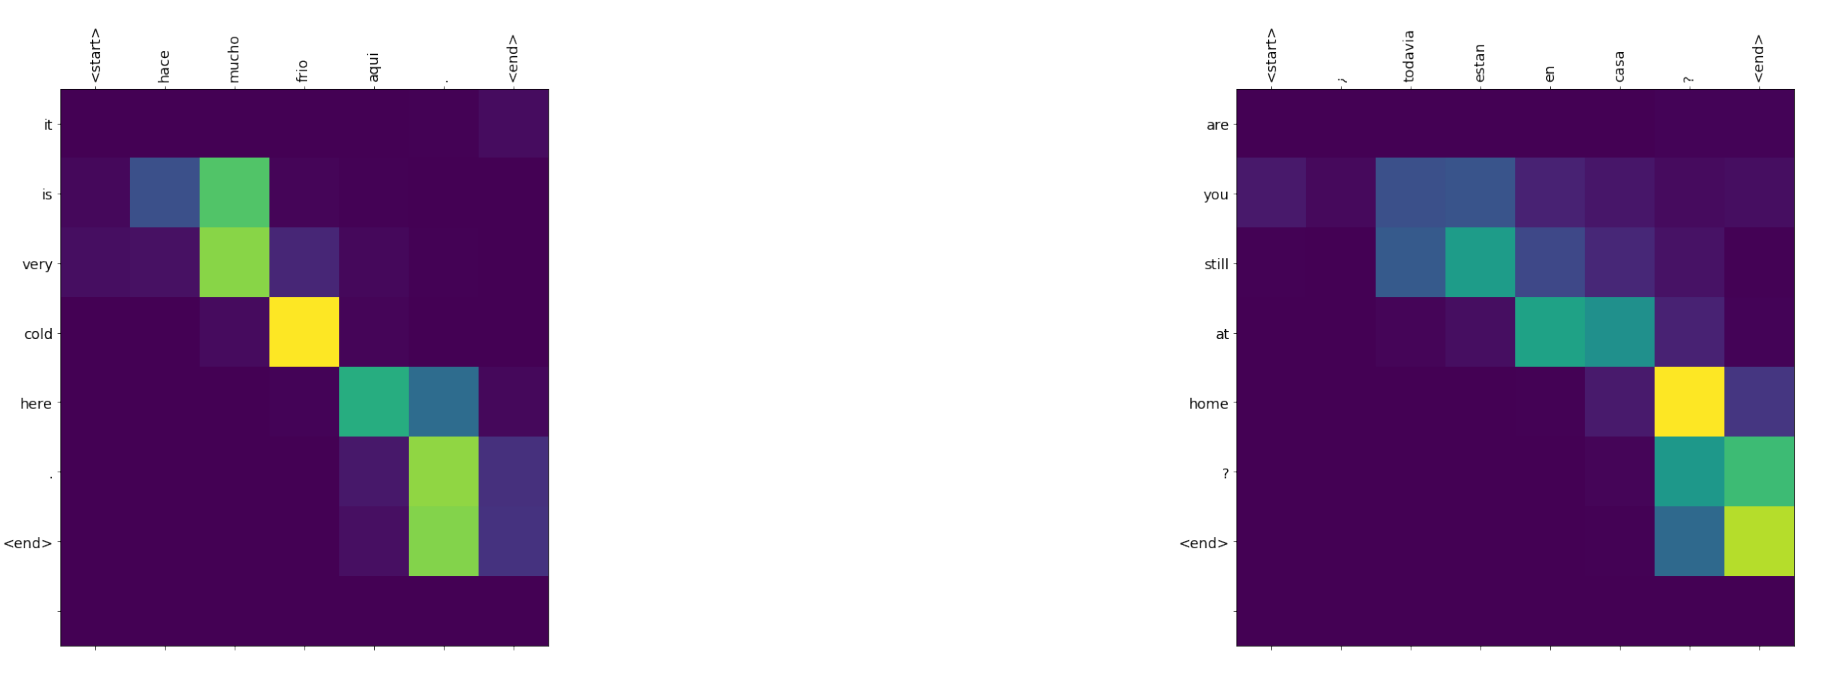
\includegraphics[width=\textwidth]{murphy_15_19.png} \\

\scriptsize Source: Murphy, Fig. 15.19 \normalsize
\end{center}
\caption{Attention score examples in English--Spanish translation}
\label{fig:murphy_15_19}
\end{figure}

\subsection*{Multi-Headed Attention}

Multi-headed attention is simply the use of multiple ''attention heads'' on the same input, as illustrated in Figure~\ref{fig:murphy_15_24}. Here, each of the queries, keys and values is first passed through a dense layer without activation function, that is, they are simply multiplied by weights, and then passed into multiple parallel attention units. The outputs of each attention unit are simply concatenated and then adjusted in dimensionality by yet another dense layer, again without activation function. Because a dense layer without activation function is simply a matrix product, multi-headed attention is defined simply as:

\begin{align*}
\operatorname{MultiHead}(Q, K, V) &= W_o \operatorname{Concat} (h_1, \ldots h_h) = W_o \begin{pmatrix} h_1 \\ \vdots \\ h_n \end{pmatrix} 
\intertext{where each head $h_i$ is defined as:}
h_i &= \operatorname{Attn}(QW_i^{(Q)}, KW_i^{(K)}, VW_i^{(V)})
\end{align*}
and $W_i^{(Q)}, W_i^{(K)}, W_i^{(V)},$ and $W^{(O)}$ are trainable weight matrices.

\begin{figure}
\begin{center}
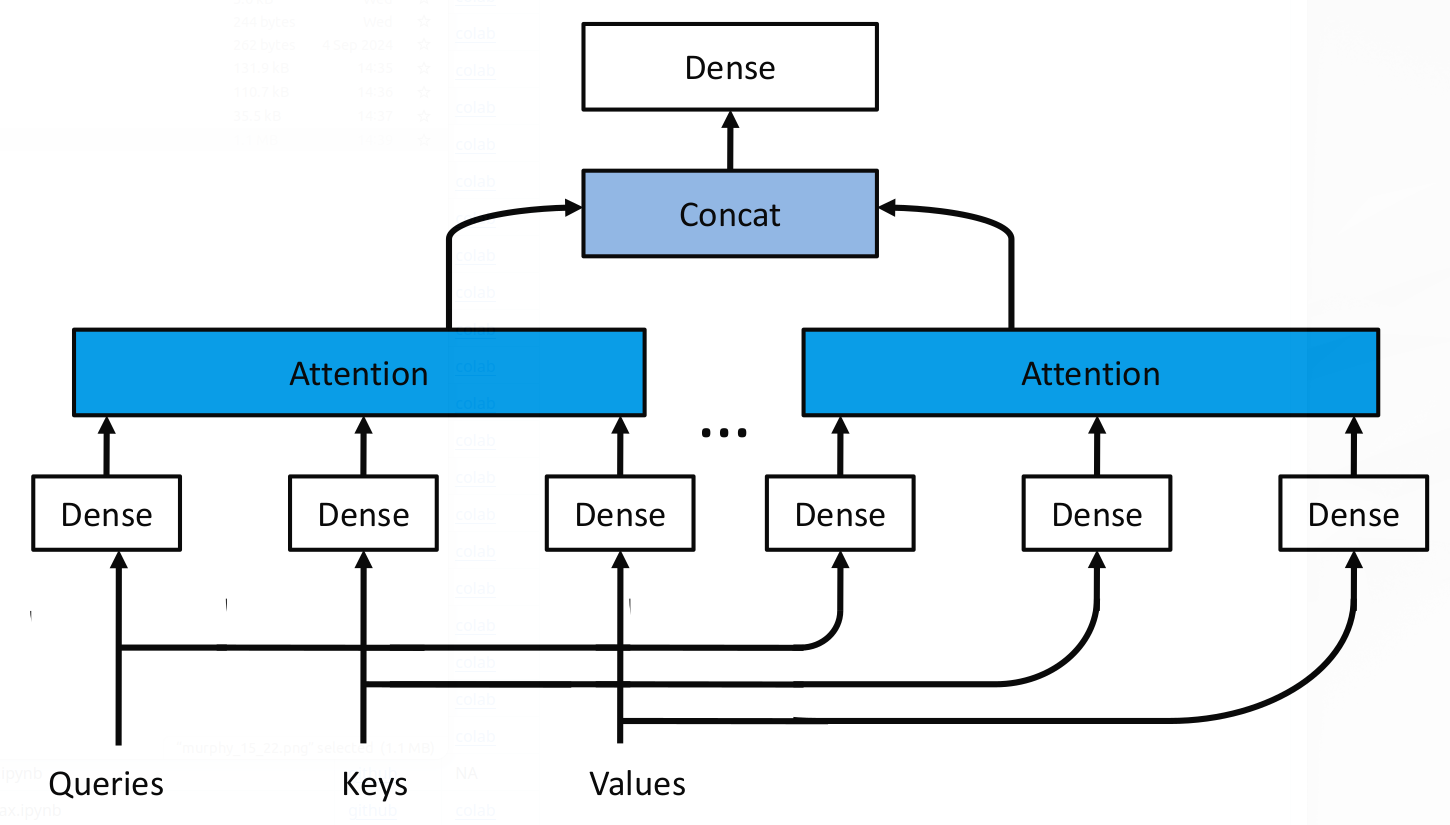
\includegraphics[width=.8\textwidth]{murphy_15_24.png} \\

\scriptsize Source: Murphy, Fig. 15.24 \normalsize
\end{center}
\caption{Multi-headed attention}
\label{fig:murphy_15_24}
\end{figure}

\subsection*{Self-Attention}

The example in Figure~\ref{fig:murphy_15_18} showed the decoder paying attention to the hidden states of the encoder. However, the encoder can also be configured to pay attention to itself. In \emph{self-attention}, the query vector, the set of keys and set of values come from the same model, that is, either the encoder or the decoder. Self-attention is defined as follows and Figure~\ref{fig:murphy_15_23} provides an illustration of a sequence encoder paying attention to itself, that is, to it's own hidden states. In the panel on the left, the encoder at the word ''it'' pays attention to the word ''animal'', that is, the hidden state at ''it'' depends on the hidden state after ''animal''. In the panel on the right, the encoder at ''it'' pays attention to the word ''street''. This example illustrates how self-attention can help remove referential ambiguity and determine word meaning depending on context. 

\begin{align*}
y_i = \operatorname{Attn}(x_i, X, X)
\end{align*}
Where $y_1$ is output $i$, $x_i$ is input $i$, and the matrix $X$ is the matrix of all $n$ inputs in the sequence. 

\begin{figure}
\begin{center}
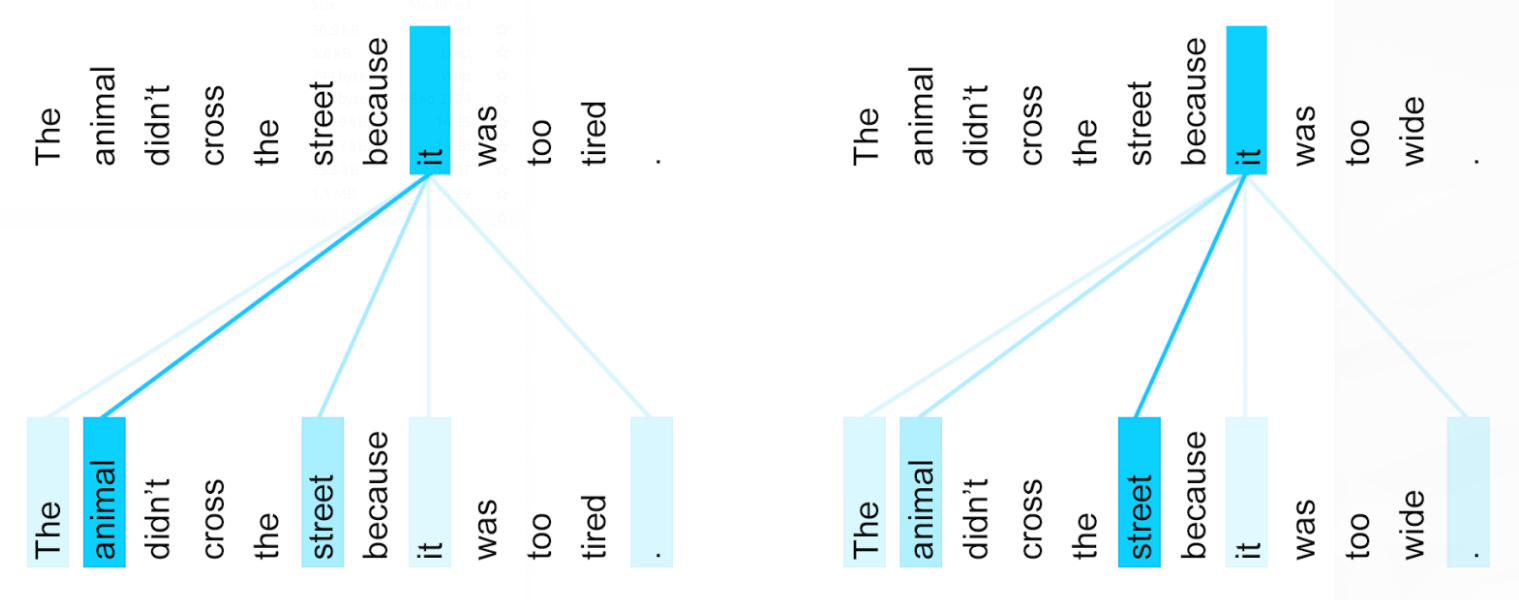
\includegraphics[width=\textwidth]{murphy_15_23.png} \\

\scriptsize Source: Murphy, Fig. 15.23 \normalsize
\end{center}
\caption{Self-encoder in attention in sequence processing}
\label{fig:murphy_15_23}
\end{figure}


\subsection*{Positional Encoding}

One problem with attention as described above is that it is independent of the word order. To take word order into account, the relative position of a word must be encoded and this \emph{positional encoding}\index{Positional encoding} is then added to the word embedding. A typical positional encoding uses sine and cosine functions as follows:

\begin{align}
&p_{i, 2j} = \sin \left( \frac{i}{C^{2j/d}} \right), \ p_{i, 2j+1} = \cos \left( \frac{i}{C^{2j/d}} \right) \ \forall j \in [1 \ldots d/2]  \label{eq:pos_encoding}
\end{align}

where $d$ is the chosen dimensionality of the positional encoding and  $C$ is the maximum sequence length. Each row $p_i$ is a real-valued vector representing its relative position in the sequence. For example, if $d=4$ the i-th row is:

\begin{align*}
&p_i = [ \sin(\frac{i}{C^{0/4}}), \cos(\frac{i}{C^{0/4}}), \sin(\frac{i}{C^{2/4}}), \cos(\frac{i}{C^{2/4}}) ]
\end{align*}

The positional embeddings $P$ are combined with embeddings $X$ through addition:
\begin{align}
&\operatorname{POS}(\operatorname{Embed}(X)) = X + P \label{eq:pos_encoding2}
\end{align}

\begin{figure}
\begin{center}
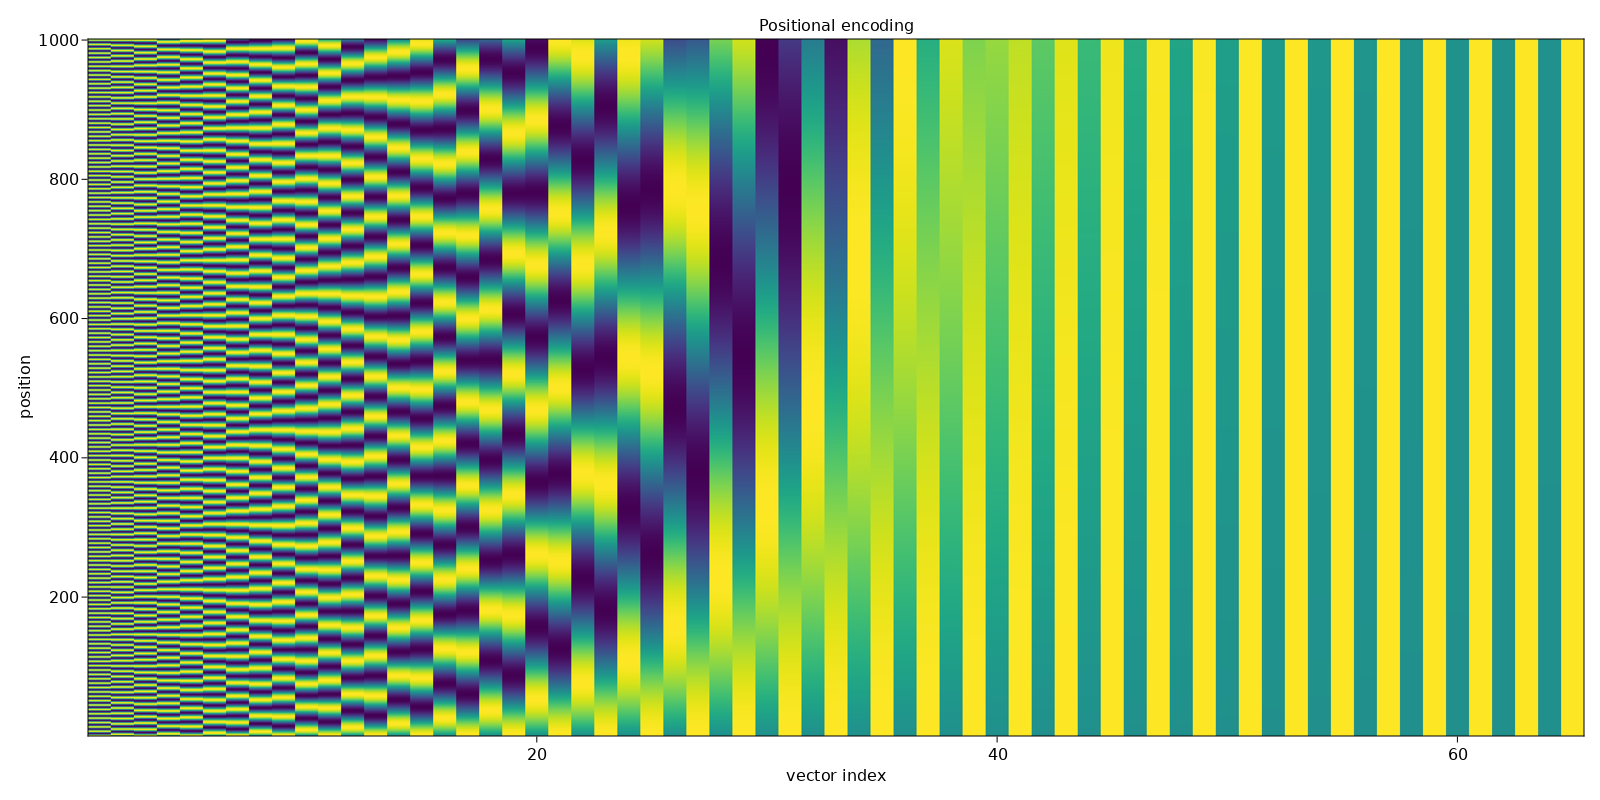
\includegraphics[width=.8\textwidth]{Positional_encoding.png} \\

\scriptsize Source: \url{https://commons.wikimedia.org/wiki/File:Positional_encoding.png} \normalsize
\end{center}
\caption{Positional encoding example}
\label{fig:positional_encoding}
\end{figure}

Figure~\ref{fig:positional_encoding} illustrates such a positional encoding graphically. Each row in the diagram represents one numerical position that is encoded as the row vector of numbers in that row. It is evident that each row is a unique row vector. The advantage over using sine and cosine functions, rather than binary numbers or integers is that they can be easily added to word embeddings, and, in contrast to integers or boolean numbers, can be immediately provided as input to a neural network. 

Positional encoding using the sine/cosine scheme in Equation~\ref{eq:pos_encoding} is implemented  in Tensorflow/Keras as an embedding layer with fixed weights, that is, the weights are determined by the sine and cosine functions of their position. The following Python code block defines a function that returns the embedding/encoding matrix according to Equation~\ref{eq:pos_encoding}:

\begin{pythoncode}
import numpy as np

def position_encoding_matrix(seq_len, d, C=10000):
    P = np.zeros((seq_len, d))
    for i in range(seq_len):
        for j in np.arange(int(d / 2)):
            denominator = np.power(C, 2 * i / d)
            P[i, 2 * j] = np.sin(i / denominator)
            P[i, 2 * j + 1] = np.cos(i / denominator)
    return P
\end{pythoncode}

The next code block then defines a custom Keras layer that combines positional and token embeddings in an additive way according to Equation~\ref{eq:pos_encoding2}:

\begin{pythoncode}
class TokenAndPositionEmbedding(layers.Layer):
    def __init__(self, maxlen, vocab_size, embed_dim):
        super().__init__()
        # Generate the positional encoding weights
        position_embedding_matrix = \
            position_encoding_matrix(maxlen, embed_dim)
        # Trainable token embedding layer
        self.token_emb = layers.Embedding(
            input_dim=vocab_size, 
            output_dim=embed_dim)
        # Positional embedding with positional 
        # encoding weights is not trainable
        self.pos_emb = layers.Embedding(
            input_dim=maxlen, 
            output_dim=embed_dim,
            weights=[position_embedding_matrix],
            trainable=False)

    def call(self, x):
        maxlen = tf.shape(x)[-1]
        positions = tf.range(0, maxlen, 1)
        # Return token plus position embedding
        return self.token_emb(x) + self.pos_emb(positions)
\end{pythoncode}

\section{Transformers}

Transformers\index{Transformer} are defined as sequence-to-sequence models that use multi-headed self-attention in both the encoder and decoder. In pseudo-code, an encoder block is defined as, where X is the input sequence and the feed-forward network is a series of dense layers.

\begin{textcode}
def EncoderBlock(X):
  Z = LayerNorm(MultiHeadAttn(Q = X, K = X, V = X) + X)
  E = LayerNorm(FeedForward(Z) + Z)
  return E
\end{textcode}

The entire encoder is then defined as a word and positional embedding, followed by a set of encoder blocks in a chain or series where the output of one encoder block is the input to the next one. 

\begin{textcode}
def Encoder(X, N):
  E = POS(Embed(X))
  for n in range(N):
    E = EncoderBlock(E)
  return E
\end{textcode}

Figure~\ref{fig:transformerencoder} shows a single encoder block schematically, but note the diagram omits the additions (''bypass'') and layer normalizations. 

\begin{figure}
\centering
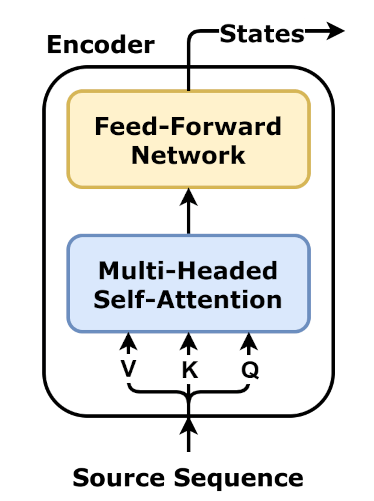
\includegraphics[height=2in]{Transformer,_one_encoder_block.png} \\

\scriptsize \url{https://commons.wikimedia.org/wiki/File:Transformer,_one_encoder_block.png}\normalsize
\caption{Transformer encoder block}
\label{fig:transformerencoder}
\end{figure}

In a similar way, the decoder block of a transformer is defined in pseudo-code as follows where Y is the target or output sequence and E is the state of an encoder block. Again, the feed-forward network is a series of dense layers. Figure~\ref{fig:transformerdecoder} shows a single decoder block schematically, but again the diagram omits the additions (''bypass'') and layer normalizations.

\begin{textcode}
def DecoderBlock(Y, E):
  Z = LayerNorm(MultiHeadAttn(Q = Y, K = Y, V = Y) + Y)
  Z' = LayerNorm(MultiHeadAttn(Q = Z, K = E, V = E) + Z)
  D = LayerNorm(FeedForward(Z') + Z')
  return D
\end{textcode}

The entire decoder is defined as a word and positional embedding of the target sequence, followed by a series or chain of decoder blocks, where the output of one decoder is the input of the next:

\begin{textcode}
def Decoder(Y, E, N):
  D = POS(Embed(Y))
  for n in range(N):
    D = DecoderBlock(D,E)
  return D
\end{textcode}

\begin{figure}
\begin{center}
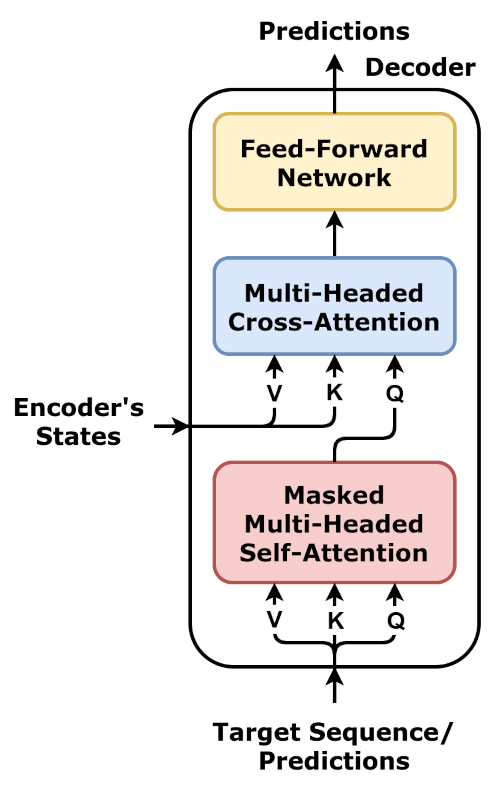
\includegraphics[height=3in]{Transformer,_one_decoder_block.png} \\

\scriptsize \url{https://commons.wikimedia.org/wiki/File:Transformer,_one_decoder_block.png}\normalsize
\end{center}
\caption{Transformer decoder block}
\label{fig:transformerdecoder}
\end{figure}

Putting the encoder and decoder together yields the complete transformer, shown schematically in Figure~\ref{fig:transformer}. This diagram contains the additive elements and the layer normalizations shown in the pseudocode above. 

One of the key advantages of the transformer over other RNN is the fact that it does not require sequential training of a sequence. A transformer can be trained on an entire input and output sequence in one parallel operation, instead of sequentially training the model for each unfolded step as is the case for LSTM or GRU based RNNs.

\begin{figure}
\centering

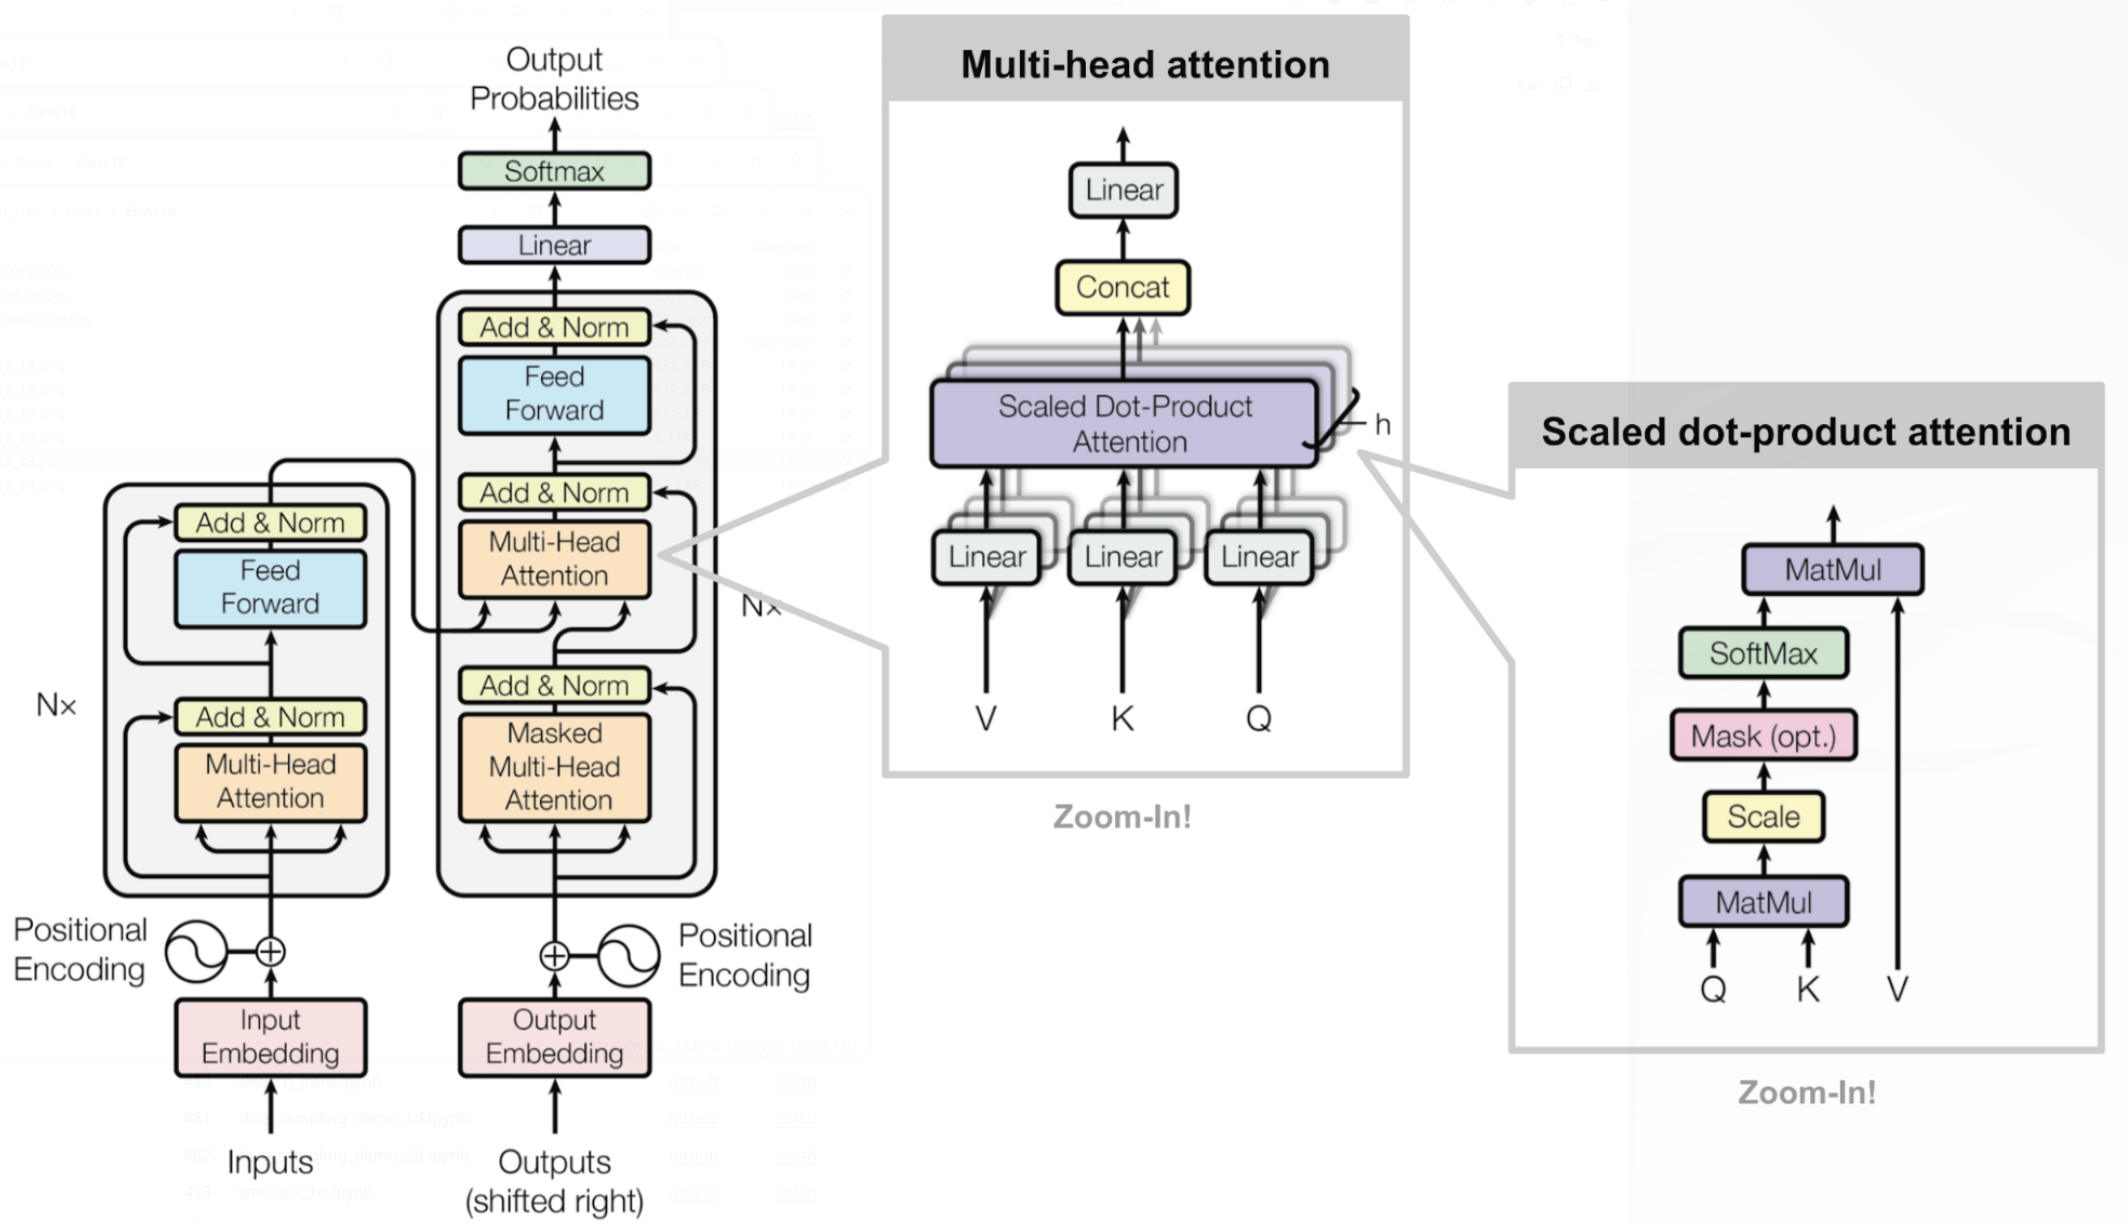
\includegraphics[width=\textwidth]{murphy_15_26.png} \\

\scriptsize Source: Murphy, Fig. 15.26 \normalsize
\caption{Transformer}
\label{fig:transformer}
\end{figure}

A transformer encoder block is easily implemented in Python, as shown in the following code block that defines a transformer as a custom Keras layer. In contrast to the diagram and schematic description, the code below adds dropout layers for regularization and includes the additive ResNet like architecture in the transformer:

\begin{pythoncode}
class TransformerBlock(layers.Layer):
    def __init__(self, embed_dim, num_heads, ff_dim, rate=0.1):
        super().__init__()
        self.att = layers.MultiHeadAttention(num_heads, embed_dim)
        self.ffn = keras.Sequential([
                layers.Dense(ff_dim, activation="relu"),
                layers.Dense(embed_dim)])
        self.norm1 = layers.LayerNormalization()
        self.norm2 = layers.LayerNormalization()
        self.dropout1 = layers.Dropout(rate)
        self.dropout2 = layers.Dropout(rate)

    def call(self, inputs):
        att_out = self.att(inputs, inputs)
        att_out = self.dropout1(att_out)
        out1 = self.norm1(inputs + att_out)
        ffn_out = self.ffn(out1)
        ffn_out = self.dropout2(ffn_out)
        return self.norm2(out1 + ffn_out)
\end{pythoncode}

\FloatBarrier

\subsection*{ELMo}

Word representation models assign a vector of real values to each word. However, rather than simply using a learned embedding matrix that results from a specific task, word representation models such as ELMo and BERT use the hidden state of an RNN as the representation of a word. This allows the word representation to be learned in the context of prior and, if a bidirectional architecture is used, also of following words. The advantage of computing word representations in this way is that they can be trained in an unsupervised way on a large corpus of text (that is, the word/token sequence is both input and target). Such a pre-trained model of word representations can later be fine-tuned for specific tasks with specific vocabulary.


\begin{figure}
\centering
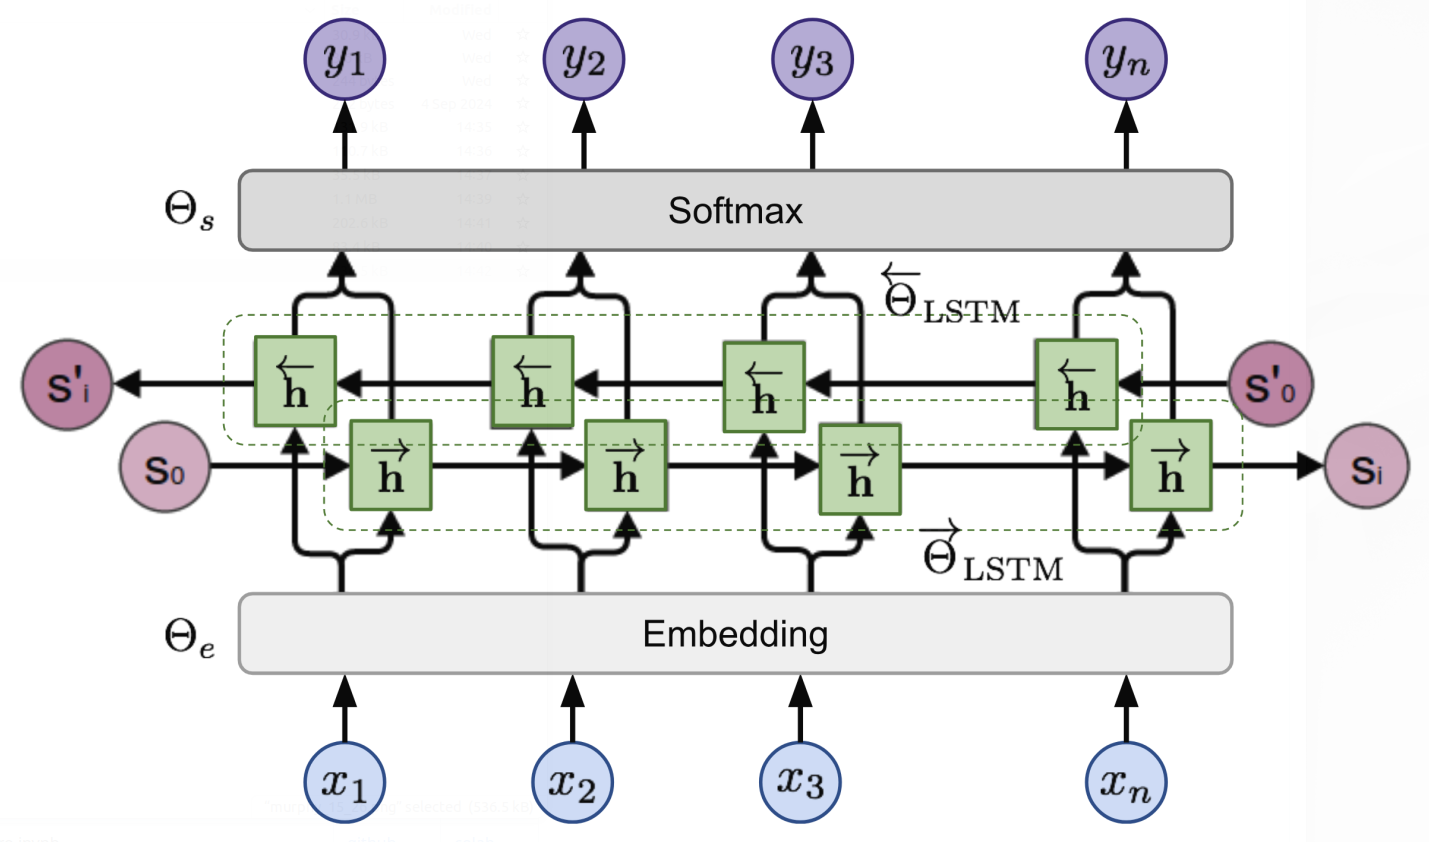
\includegraphics[width=.8\textwidth]{murphy_15_32.png} \\

\scriptsize Source: Murphy, Fig. 15.32 \normalsize
\caption{ELMo architecture}
\label{fig:murphy_15_32}
\end{figure}

The ELMo model (''Embeddings from Language Model'')\index{ELMo|see {Embeddings from Language Model}}\index{Embeddings from Language Model} uses a bi-directional multi-layer LSTM architecture shown in Figure.~\ref{fig:murphy_15_32}. For the forward LSTM, the targets are the inputs shifted to the right ($y_i = x_{i+1}$), that is, the model predicts the next token. for the backward LSTM, the targets are the inputs shifted left ($y_i = x_{i-1}$), that is, the model predicts the previous token. 

In the original ELMo implementation, words/tokens are initially embedded in an embedding matrix and the forward and backward portions of the model are 2-layered LSTMs with 4096 units (state size). The word representation is the concatenation of the embedding, both forward LSTM states, and both backward LSTM states, projected down into a 512-dimensional space. 

\subsection*{BERT}

Similar to ELMo, BERT (''Bidirectional Encoder Representations from Transformers'')\index{BERT|see {Bidirectional Encoder Representation from Transformers}}\index{Bidirectional Encoder Representation from Transformers} is a language representation model that can be trained in an unsupervised way. In contrast to ELMo, BERT uses a transformer architecture that consists only of an encoder as stacked set of transformer blocks. The architecture is shown in the left panel of Figure~\ref{fig:bert}. Similar to the ELMo architecture, BERT also uses forward and backward connections that allows word representations to be learned in the context of previous and following words. 

\begin{figure}
\centering
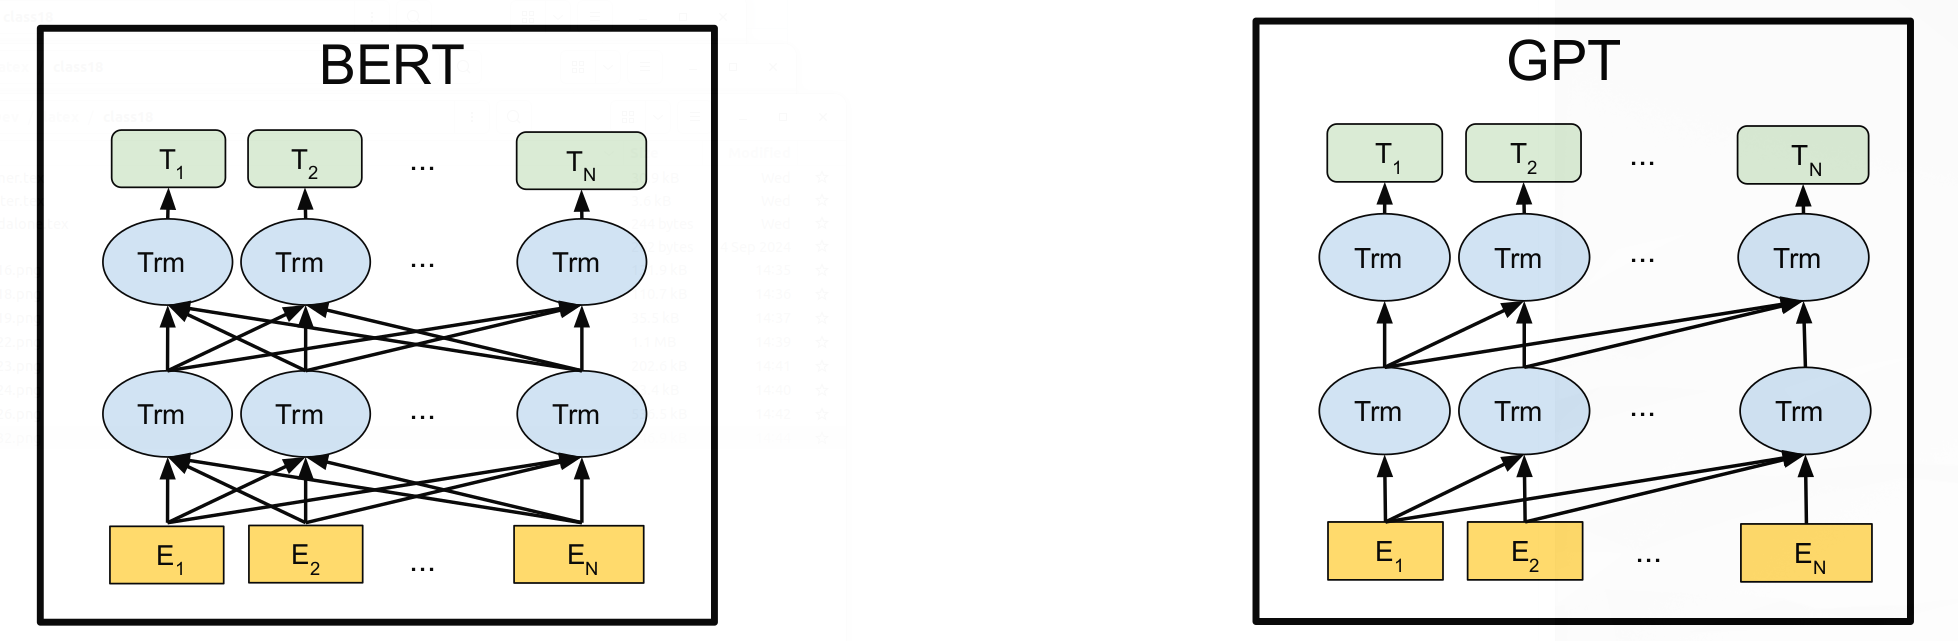
\includegraphics[width=\textwidth]{murphy_15_33.png} \\

\scriptsize Source: Murphy, Fig. 15.33 \normalsize
\caption{Comparison of BERT and GPT Architectures}
\label{fig:bert}
\end{figure}

BERT uses three embeddings for each token, as shown in Figure~\ref{fig:bertinput}. The token embeddings represent each input word/token using an embedding matrix. Note the first token [CLS] represents the task to be performed, classification. The segment embeddings represent the sentences that are separated in the sequence by a special token, here labelled [SEP]. Finally, the positional encoding indicates the relative position of the token in the sequence. The three encodings are summed for the input to the transformer. The BERT architecture is configurable in the number of transformer layers $L$ and the hidden state size $H$. There are always $H/64$ attention heads in the multi-headed attention block of the encoders. Varying these parameters yields models of different sizes and capabilities. 

\begin{figure}
\begin{center}
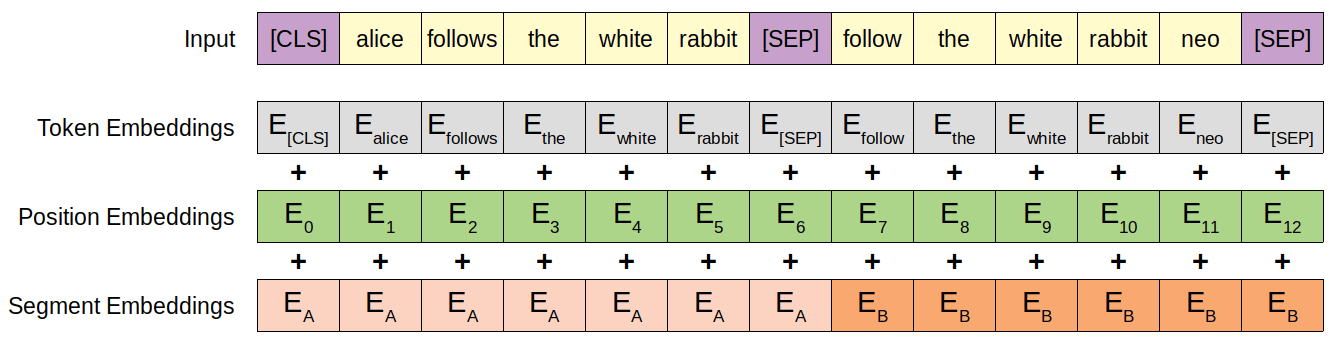
\includegraphics[width=\textwidth]{BERT_input_embeddings.png} \\

\scriptsize \url{https://commons.wikimedia.org/wiki/File:BERT_input_embeddings.png} \normalsize
\end{center}
\caption{BERT input encodings}
\label{fig:bertinput}
\end{figure}

BERT is pre-trained on two tasks, masked language modelling  and next sentence prediction. In masked language modelling (Figure~\ref{fig:bert_masked_language_modeling}), some input words are replaced by a ''mask'', that is, a special token [MASK] and the model must predict the word. The BERT model representation for the masked token is input to a feed-forward dense network for classification. Masked language modelling helps the BERT model learn words in the context of prior and later words. 

\begin{figure}
\begin{center}
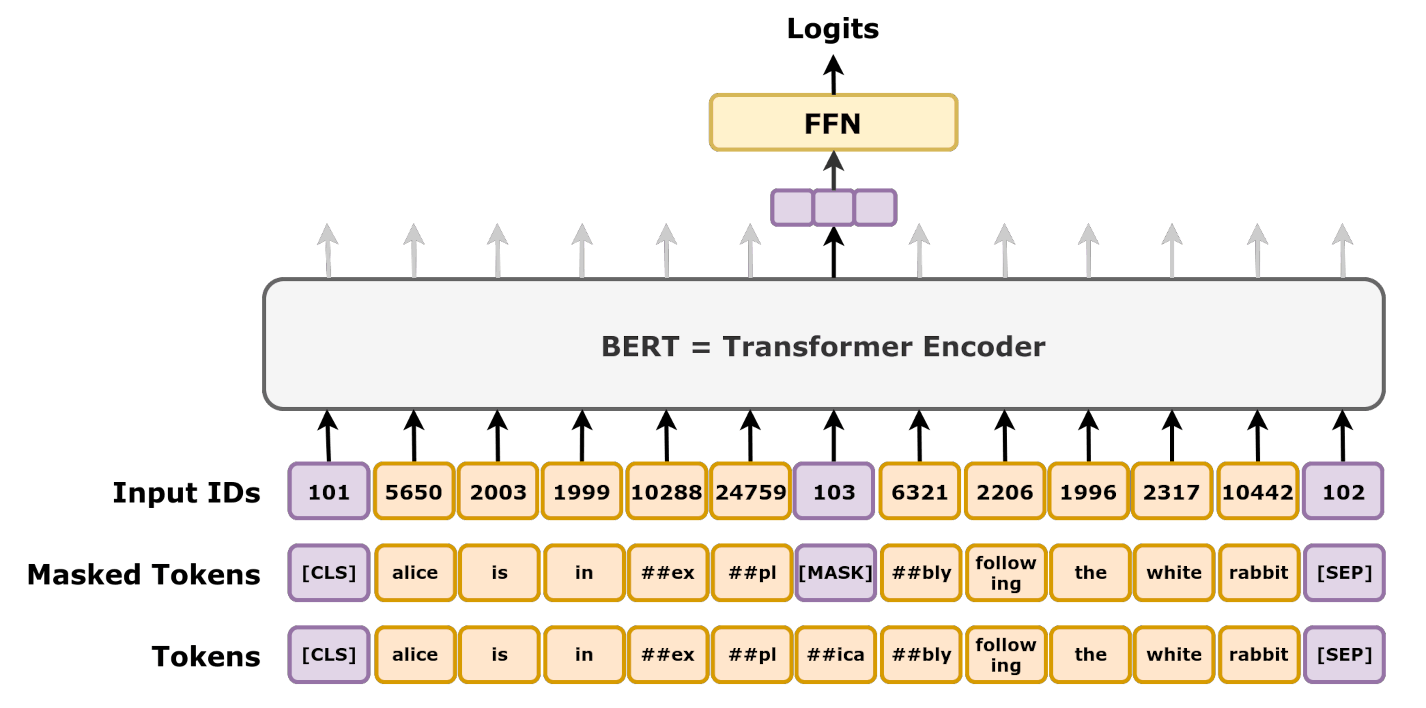
\includegraphics[width=.8\textwidth]{BERT_masked_language_modelling_task.png} \\
\tiny \url{https://commons.wikimedia.org/wiki/File:BERT_masked_language_modelling_task.png} \normalsize \\

\end{center}
\caption{BERT pre-training on masked language modelling}
\label{fig:bert_masked_language_modeling}
\end{figure}

In next sentence prediction(Figure~\ref{fig:bert_next_sentence_prediction}), the model must decide whether one sentence logically follows another, allowing the model to learn relationships between sentences, which is important for tasks such as question answering or document classification. In this task, the representation of the first token [CLS] is used as input to dense network for classification. 

\begin{figure}
\begin{center}
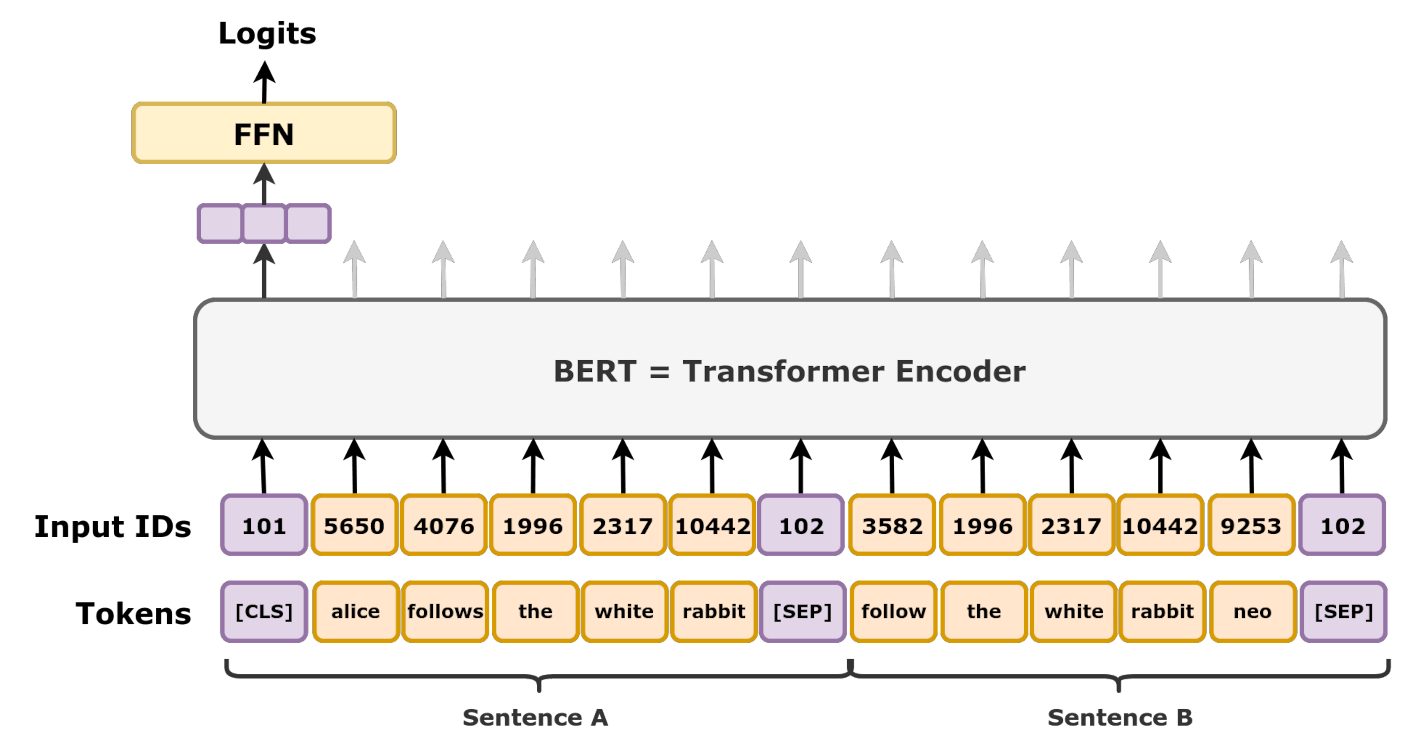
\includegraphics[width=.8\textwidth]{BERT_next_sequence_prediction_task.png} \\
\tiny \url{https://commons.wikimedia.org/wiki/File:BERT_next_sequence_prediction_task.png} \normalsize

\end{center}
\caption{BERT pre-training on next sentence prediction}
\label{fig:bert_next_sentence_prediction}
\end{figure}

After pre-training, the BERT model can be fine-tuned for specific language tasks, such as sentence classification, question answering, or part-of-speech tagging. These fine-tuning tasks and their architectures are illustrated in Figures~\ref{fig:bert_sentence_classification} to \ref{fig:bert_tagging}. In sentence classification (e.g. sentiment: positive/negative), the task representation of [CLS] is input to a dense classification network (Figure~\ref{fig:bert_sentence_classification}), while in multiple-choice question answering, the tokens in the passage represent possible answers and their representations form the input to dense layers for classification (e.g. true/false) (Figure~\ref{fig:bert_multiple_choice}). Finally, in part-of-speech tagging, the representations of all tokens are input to dense classification networks for classification (e.g. subject, object, etc.) (Figure~\ref{fig:bert_tagging}).  

\begin{figure}
\centering
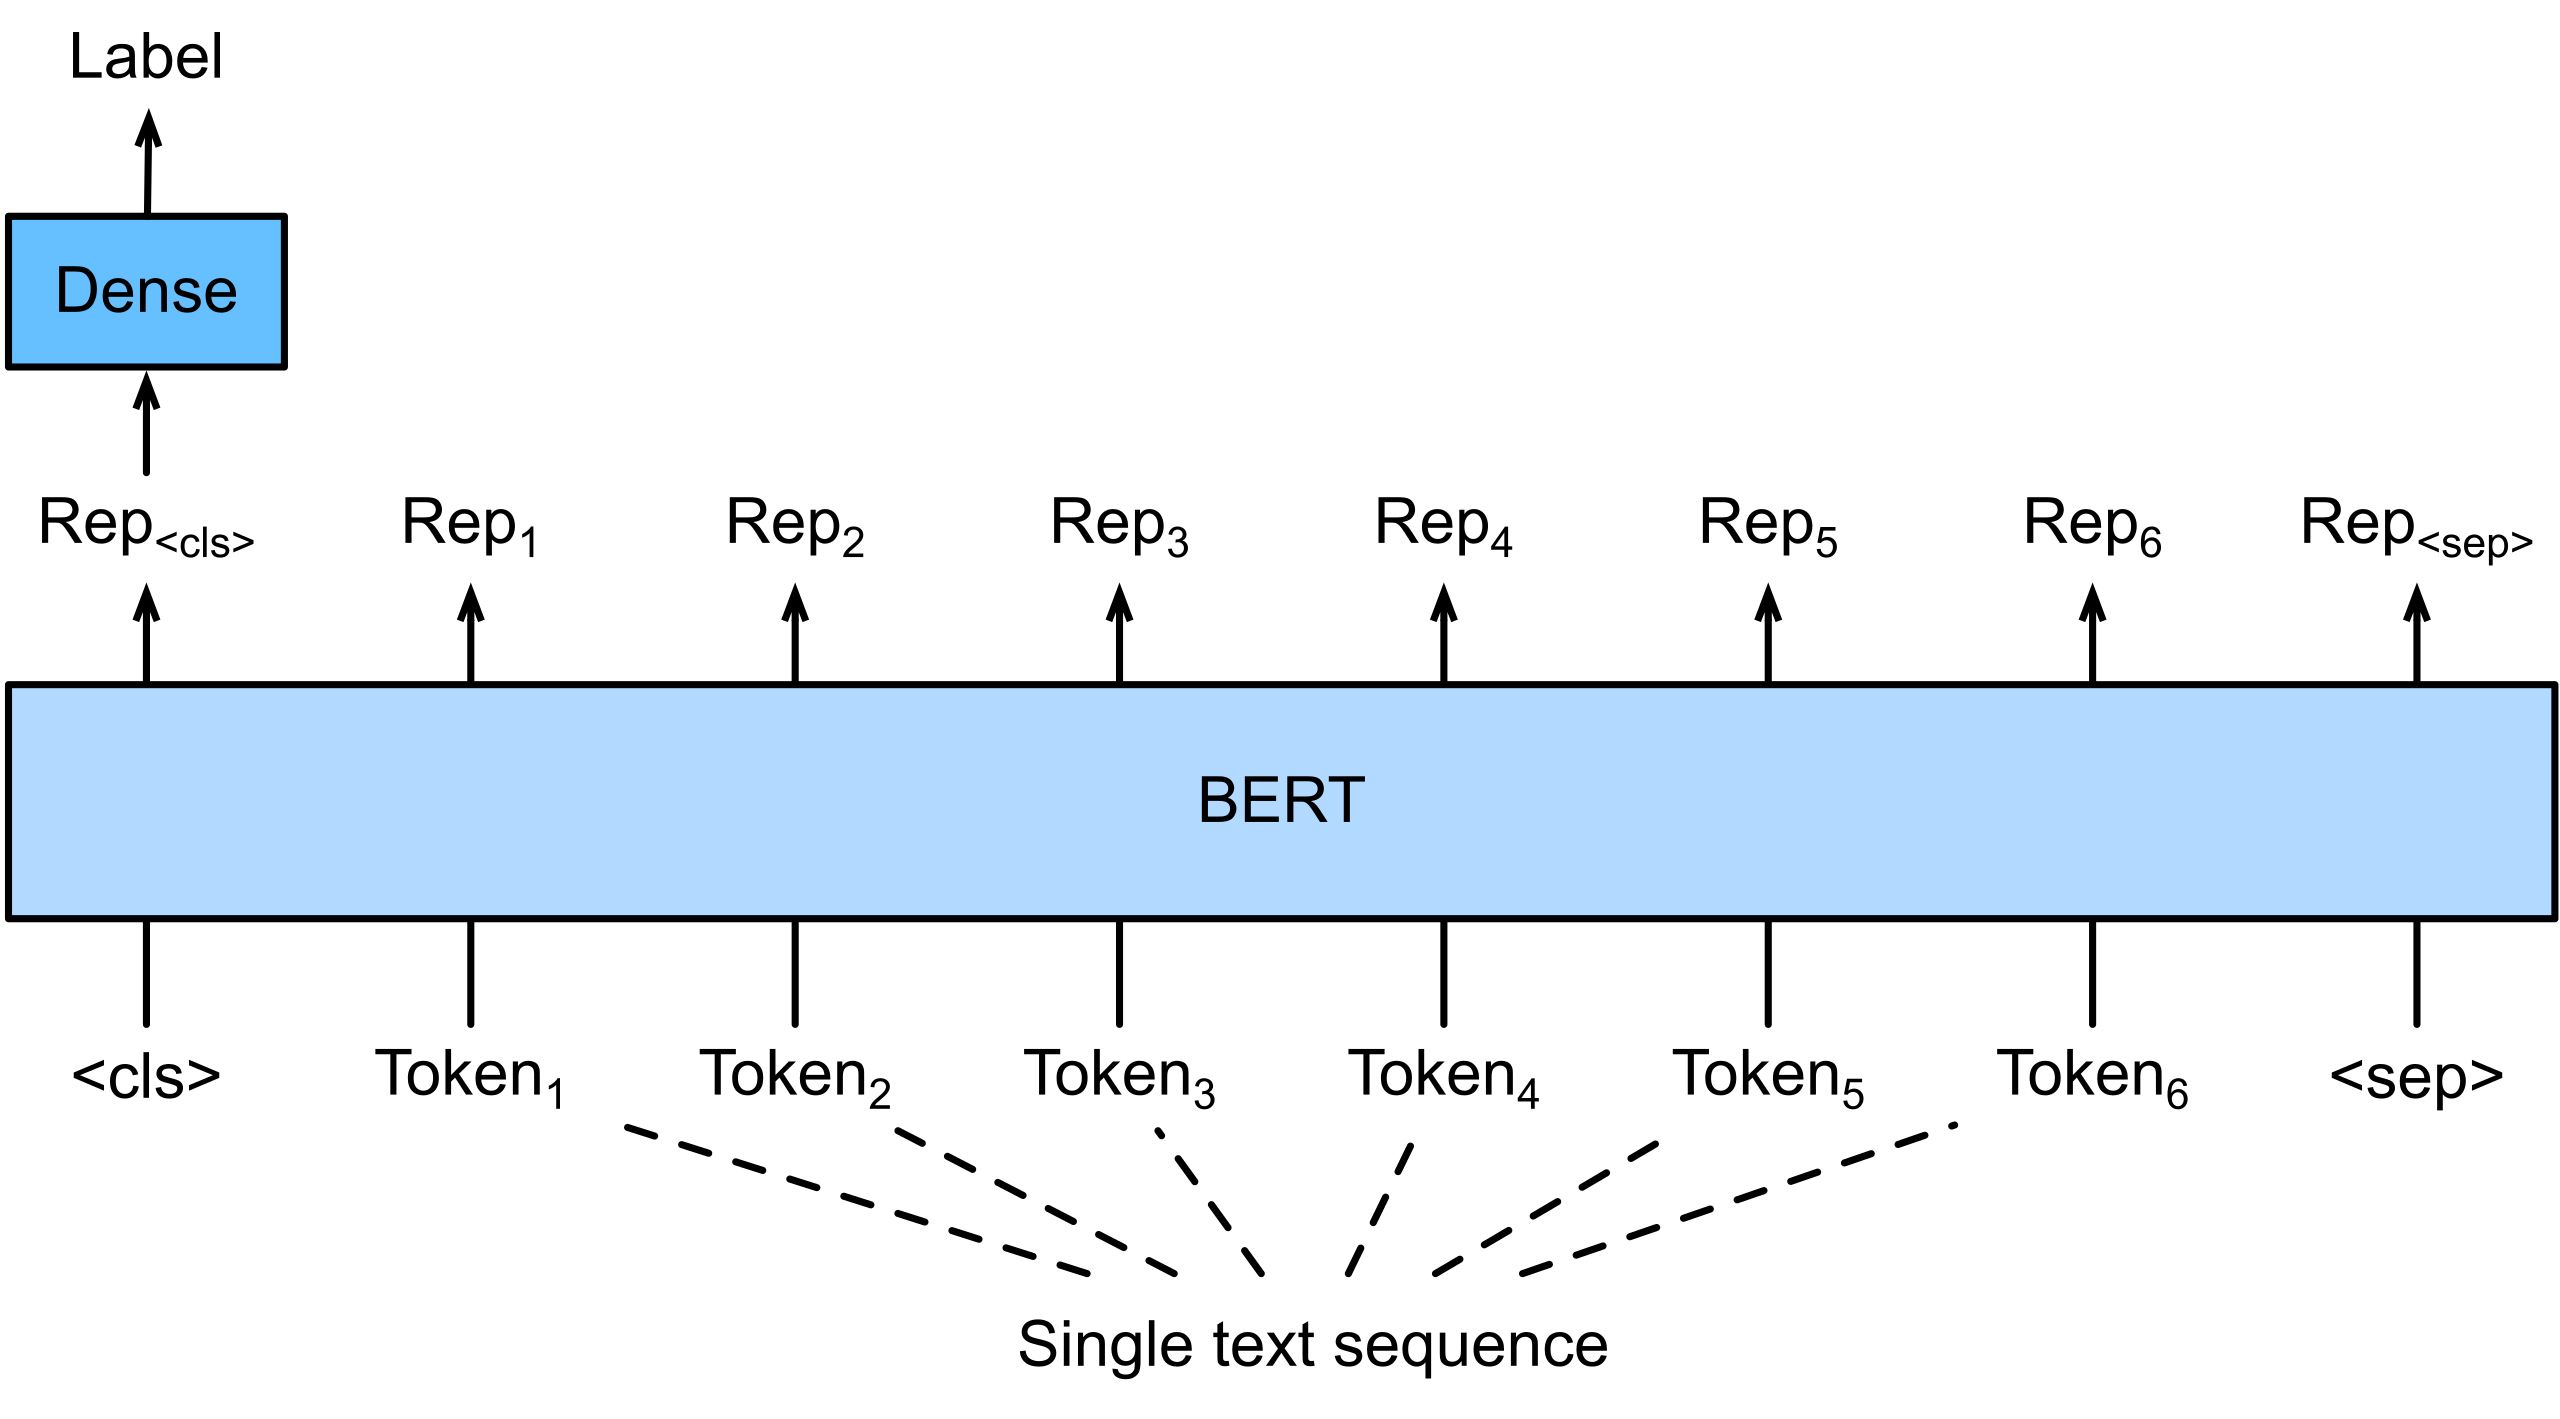
\includegraphics[width=.8\textwidth]{BERT_on_sentence_classification.svg.png} \\

\tiny \url{https://commons.wikimedia.org/wiki/File:BERT_on_sentence_classification.svg}\normalsize
\caption{BERT fine-tuning on sentence classification}
\label{fig:bert_sentence_classification}
\end{figure}

\begin{figure}
\centering
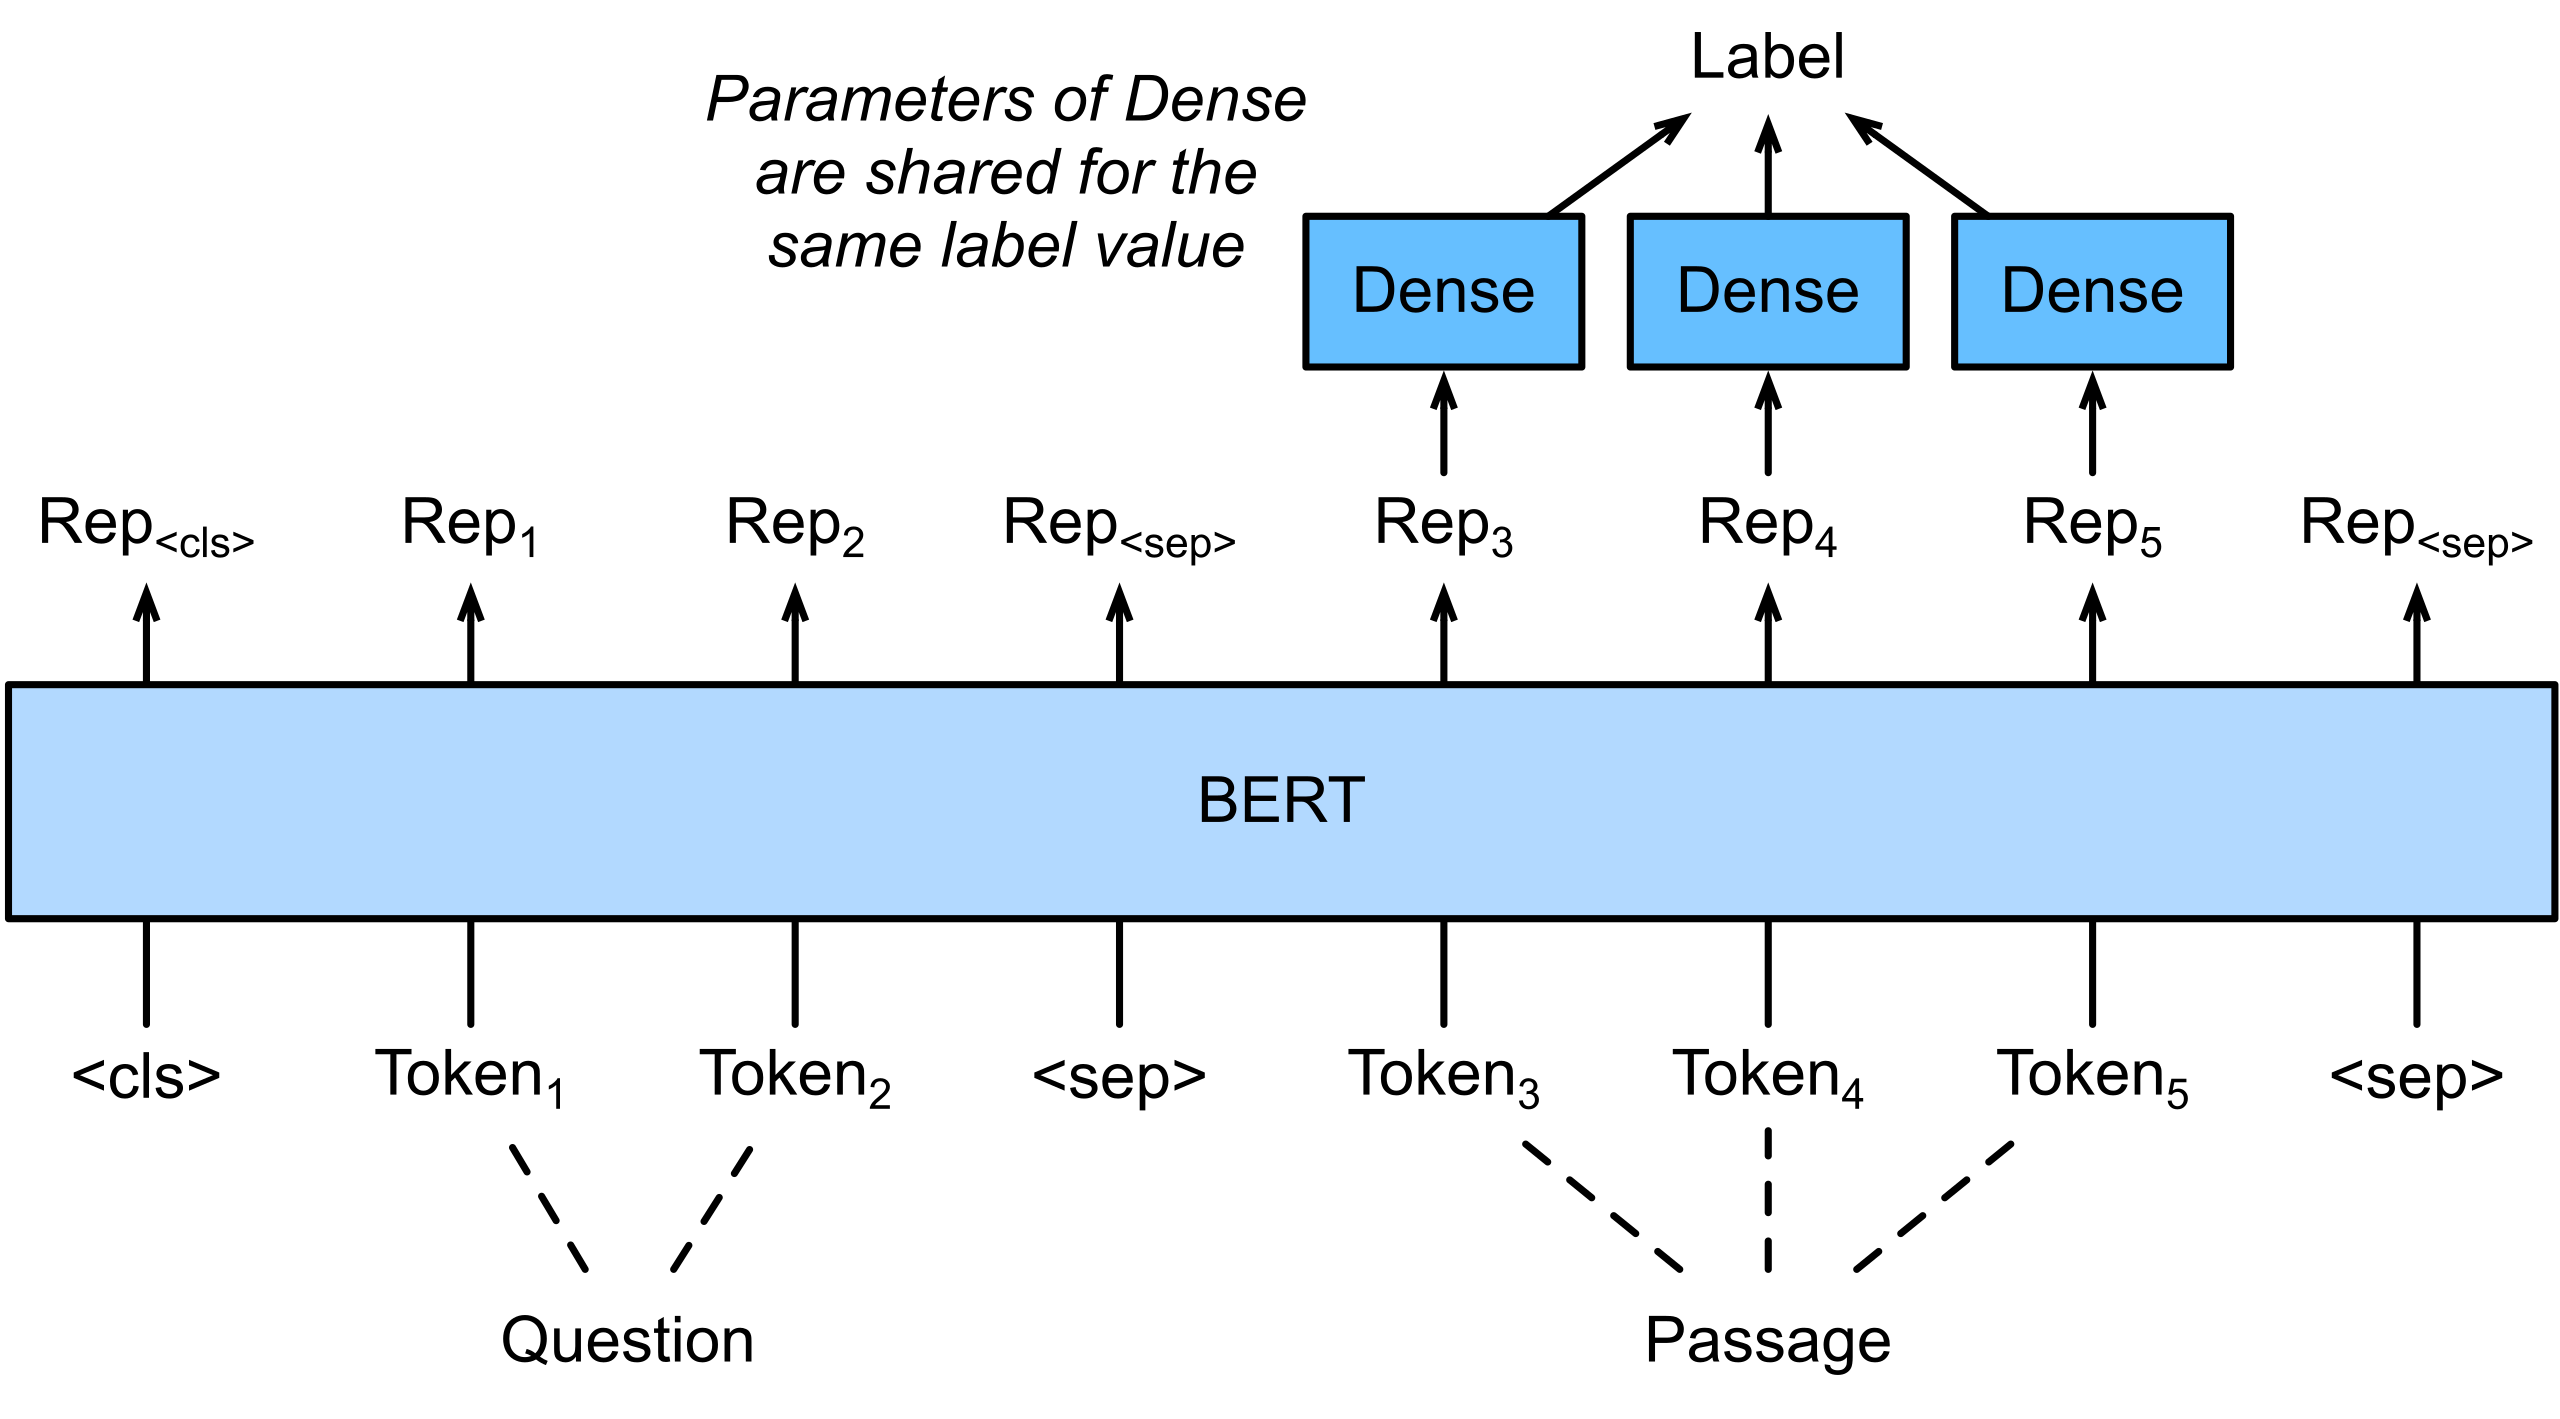
\includegraphics[width=.8\textwidth]{BERT_on_multiple-choice_question-answering.svg.png} \\

\tiny \url{https://commons.wikimedia.org/wiki/File:BERT_on_multiple-choice_question-answering.svg} \normalsize
\caption{BERT fine-tuning on multiple choice question answering}
\label{fig:bert_multiple_choice}
\end{figure}

\begin{figure}
\centering
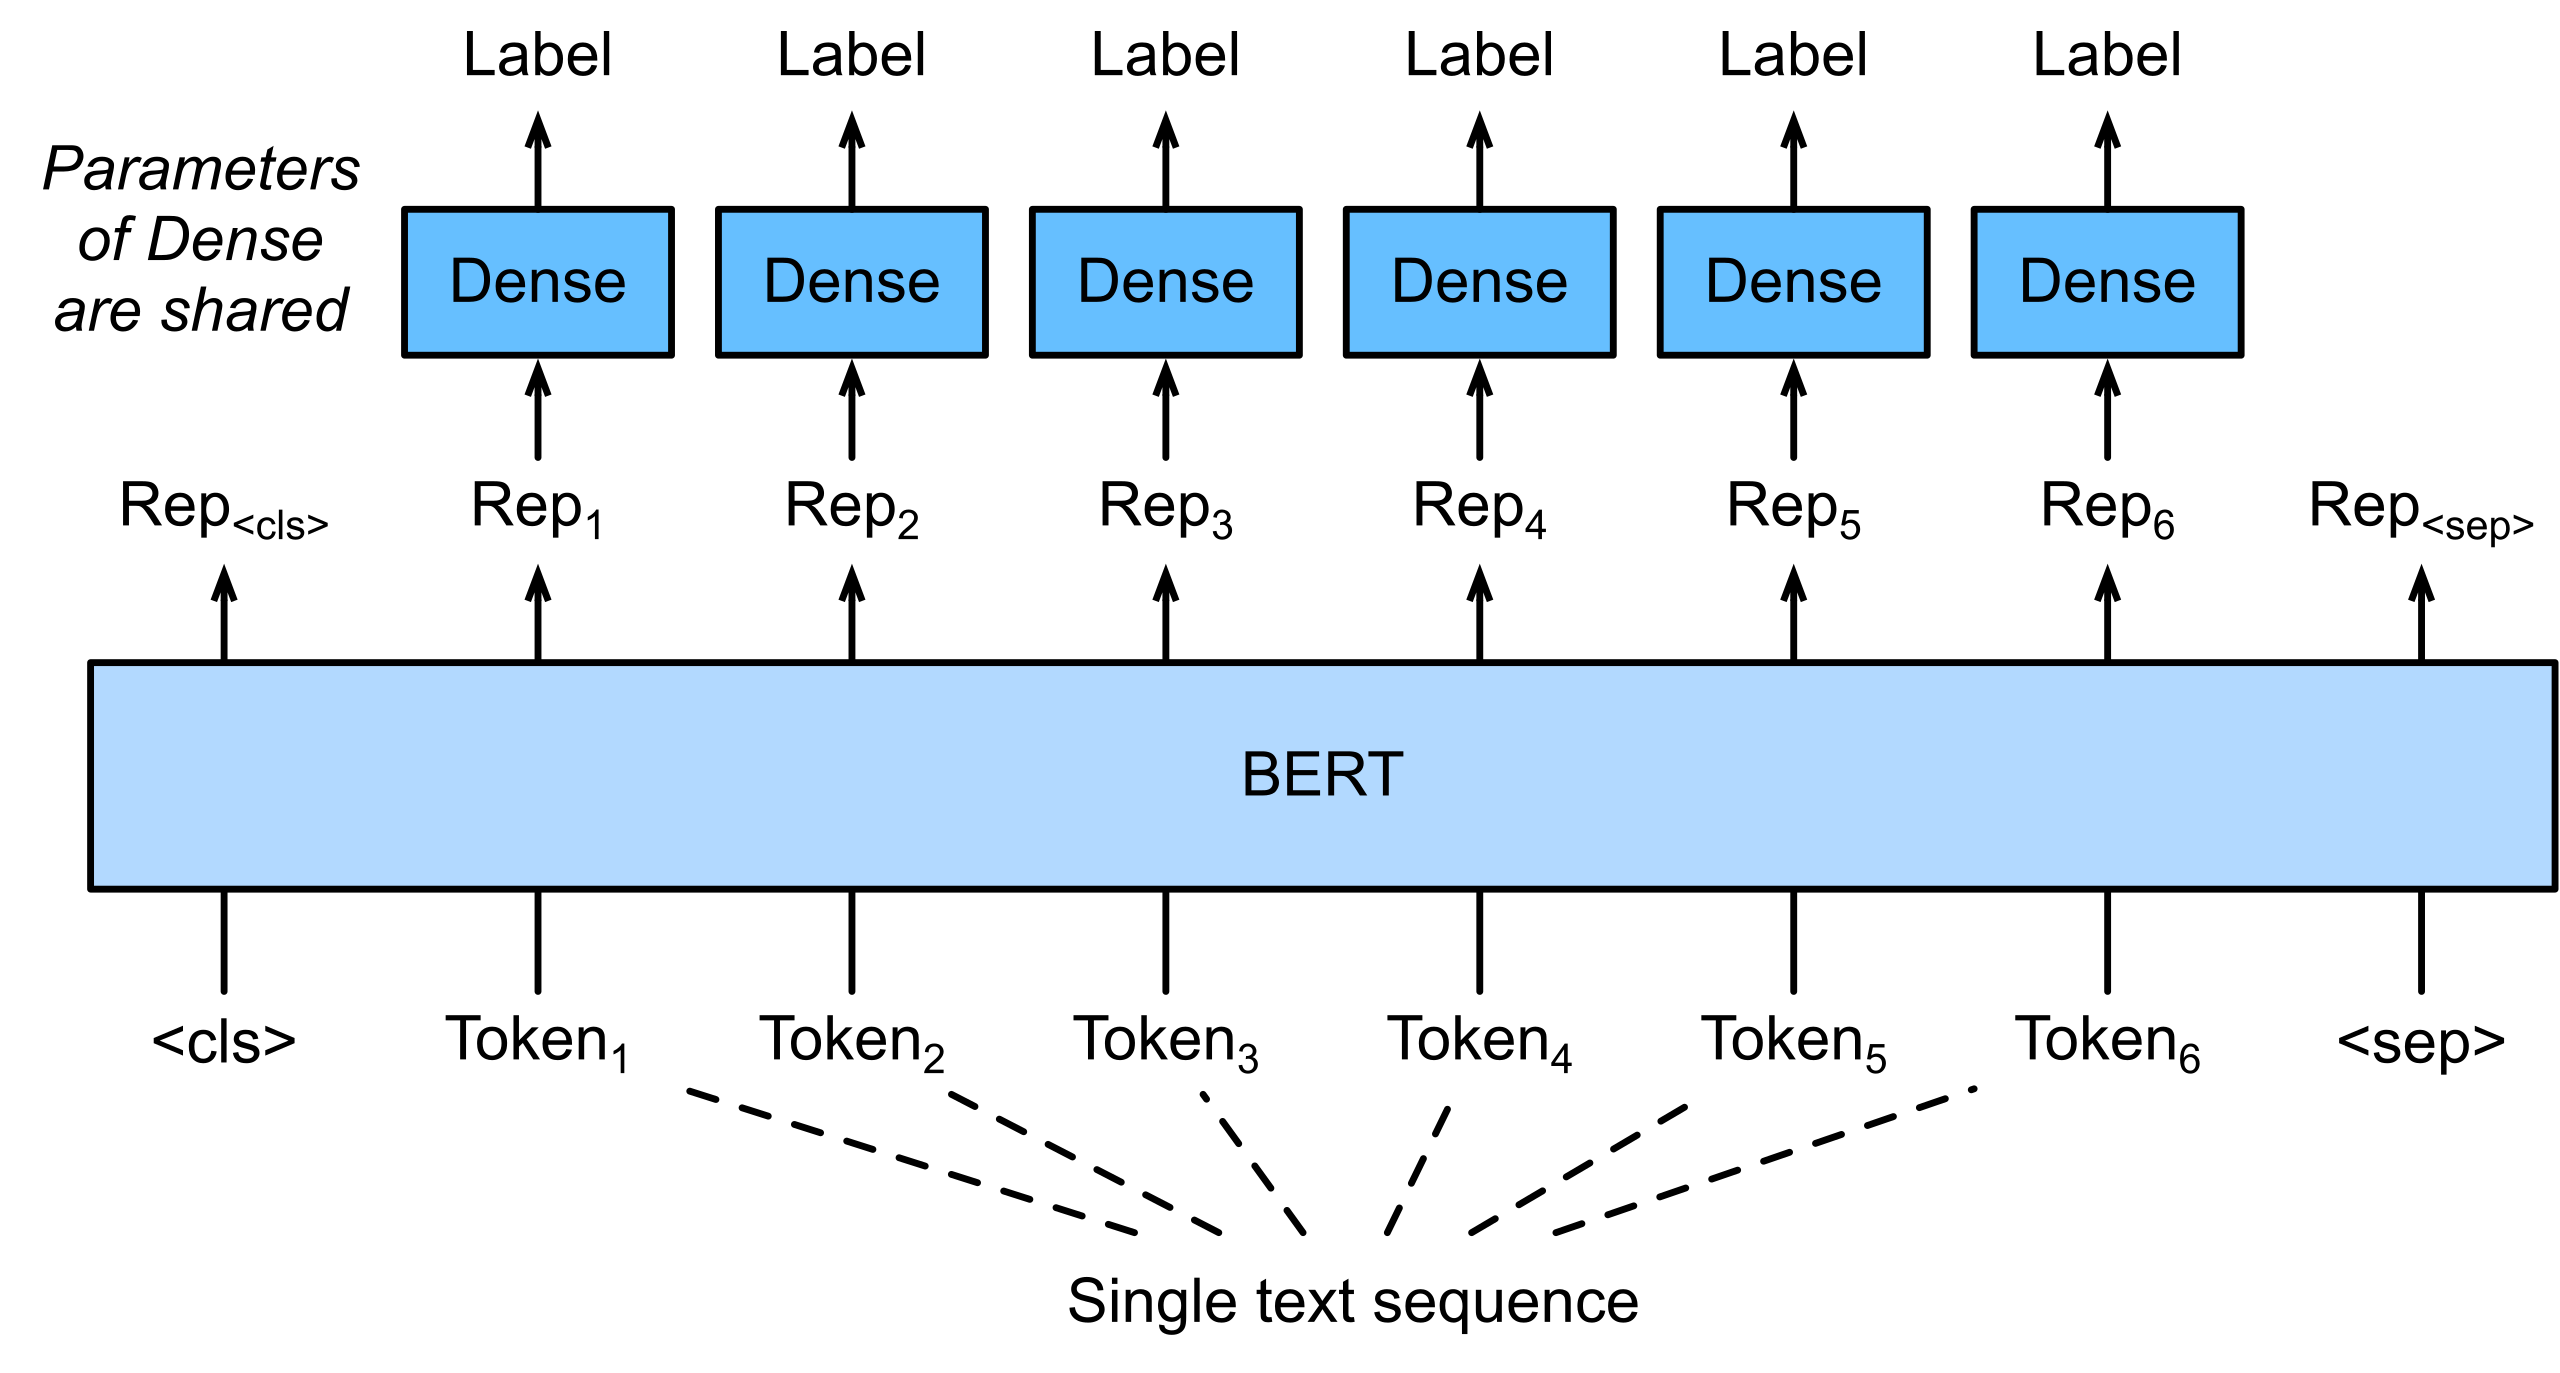
\includegraphics[width=.8\textwidth]{BERT_on_tagging.svg.png} \\

\tiny \url{https://commons.wikimedia.org/wiki/File:BERT_on_tagging.svg} \normalsize
\caption{BERT fine-tuning on part-of-speech tagging}
\label{fig:bert_tagging}
\end{figure}

\FloatBarrier


\begin{resourcebox}
The TensorFlow and Keras websites have a multitude of guides and tutorials on language processing and generation with transformers. The ones recommended below illustrate the main topics covered in this section on Transformer architectures.

\subsubsection*{Keras:}
\begin{itemize}
\item \href{https://keras.io/examples/generative/text_generation_with_miniature_gpt/}{Text generation with a miniature GPT} 
\item \href{https://keras.io/examples/nlp/text_classification_with_transformer/}{Text classification with a transformer} 
\item \href{https://keras.io/examples/nlp/neural_machine_translation_with_transformer/}{English-to-Spanish translation with seq2seq transformer} 
\item \href{https://keras.io/examples/nlp/semantic_similarity_with_bert/}{Semantic similarity with BERT} 
\end{itemize}

\subsubsection*{Tensorflow:}
\begin{itemize}
\item \href{https://www.tensorflow.org/text/tutorials/transformer}{Neural machine translation with a Transformer and Keras} 
\item \href{https://www.tensorflow.org/text/tutorials/classify_text_with_bert}{Classify text with BERT} 
\item \href{https://www.tensorflow.org/tfmodels/nlp/fine_tune_bert}{Fine-tuning a BERT model} 
\end{itemize}
\end{resourcebox}

\section{Auto-Encoders}

An auto-encoder\index{Auto-encoder} is a neural network that maps a high-dimensional input into a point in a lower dimensional embedding space or latent space. The model architecture consists of a an encoder\index{Encoder} and a decoder\index{Decoder} (Figure~\ref{fig:autoencoder}). In a simple case, these can be dense or feed-forward networks, but they may also consist of convolutional layers (and their inverse, the convolutional transpose, in the decoder) or, as seen above for sequence-to-sequence models, of RNNs. They are trained in such a way that the input is also the target output, so that encoder and decoder are trained at the same time.

\begin{figure}
\begin{center}
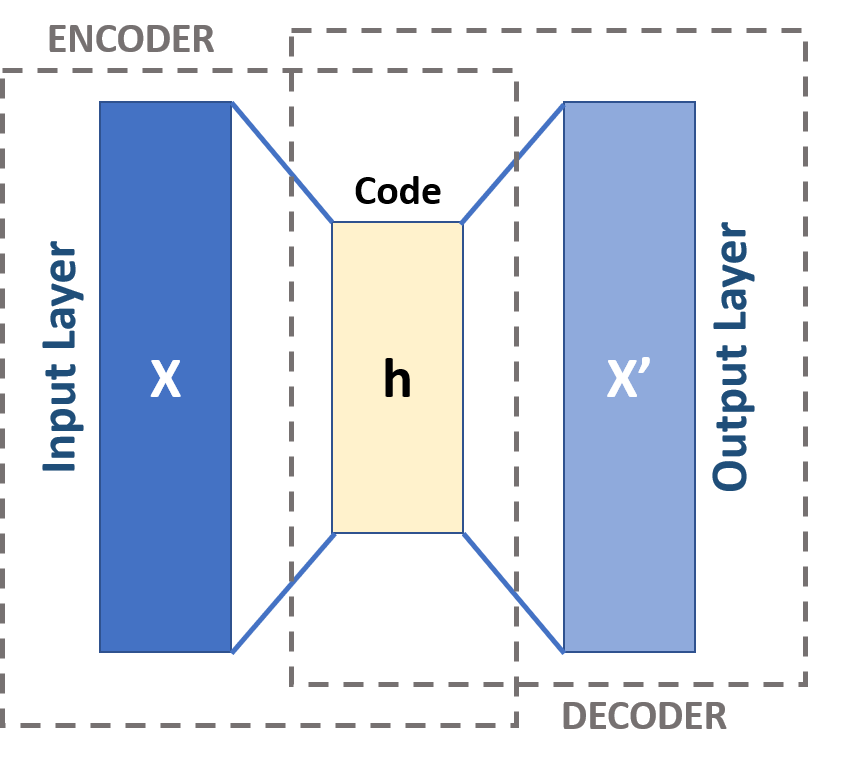
\includegraphics[height=2in]{Autoencoder_schema.png} \\

\scriptsize \url{https://commons.wikimedia.org/wiki/File:Autoencoder_schema.png} \normalsize
\caption{Autoencoder}
\label{fig:autoencoder}
\end{center}
\end{figure}

A frequent use case for auto-encoders is with image data. Figure~\ref{fig:mnist_autoencoder} shows two examples of an auto-encoder with the MNIST Fashion image data set. In the left panel (a) of the figure, the encoder is a 3-layer densely connected network with sizes 768 (input), 100, and 30 (latent space size). The top row of images shows the input, the bottom row the decoded output. The right panel (b) of the Figure uses a 3-layer CNN for encoder, also with a latent space size of 30. Larger models could be used to improve on the decoding performance. 

\begin{figure}
\begin{center}
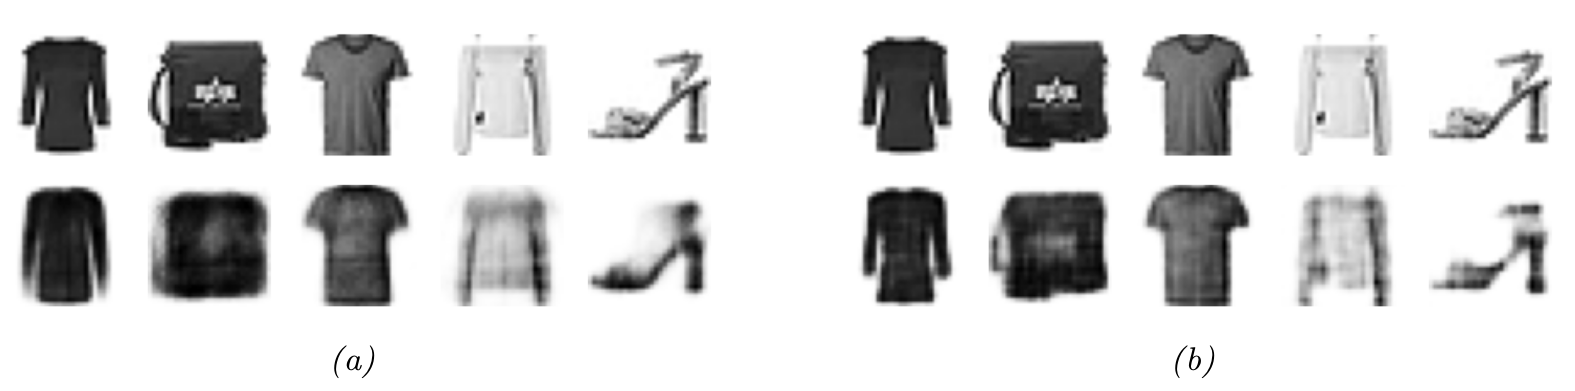
\includegraphics[width=\textwidth]{murphy_20_17.png} \\

\scriptsize Source: Murphy, Fig. 20.17 \normalsize
\caption{MNIST auto-encoder examples}
\label{fig:mnist_autoencoder}
\end{center}
\end{figure}

Auto-encoders can be viewed as data reduction models, in the same way that PCA (principal components analysis) reduces the dimensionality of the input. Similar to PCA, where observations can be located in the space spanned by the principal components, the latent space of auto-encoders can be visualized. Consider Figure~\ref{fig:mnist_autoencoder_latent_space} that shows the the first two latent dimensions and locates a variety of training observations in that space, as indicated by colours and exemplar images. The left panel shows the latent dimensions for the 3-layer densely connected network, while the right panel shows the first two latent dimensions for the 3-layer CNN. The plots show that a 30-dimensional space already provides quite clean separation of the different images and image classes and the encoder structures the latent space in such a way that related images, that is images of the same class, are co-located in the space.

Figure~\ref{fig:mnist_autoencoder_latent_space} shows some problems with auto-encoders when using them in a generative way, that is, sampling a random point in the latent space and decoding that point into output. The figure shows that the latent space is not uniformly used and is discontinuous, that is, there are large areas/volumes that do not correspond to any training data. Sampling from such areas/volumes will not yield a sensible output. Additionally, it can be seen that position of different classes of objects are well mixed in the latent space; that is, dots of different colours are frequently next to each other. This means that a small variation or ''jiggle'' when sampling is likely to yield a very output. This, too, is undesirable. In summary, auto-encoders are useful for data reduction, but not as generative models.

\begin{figure}
\begin{center}
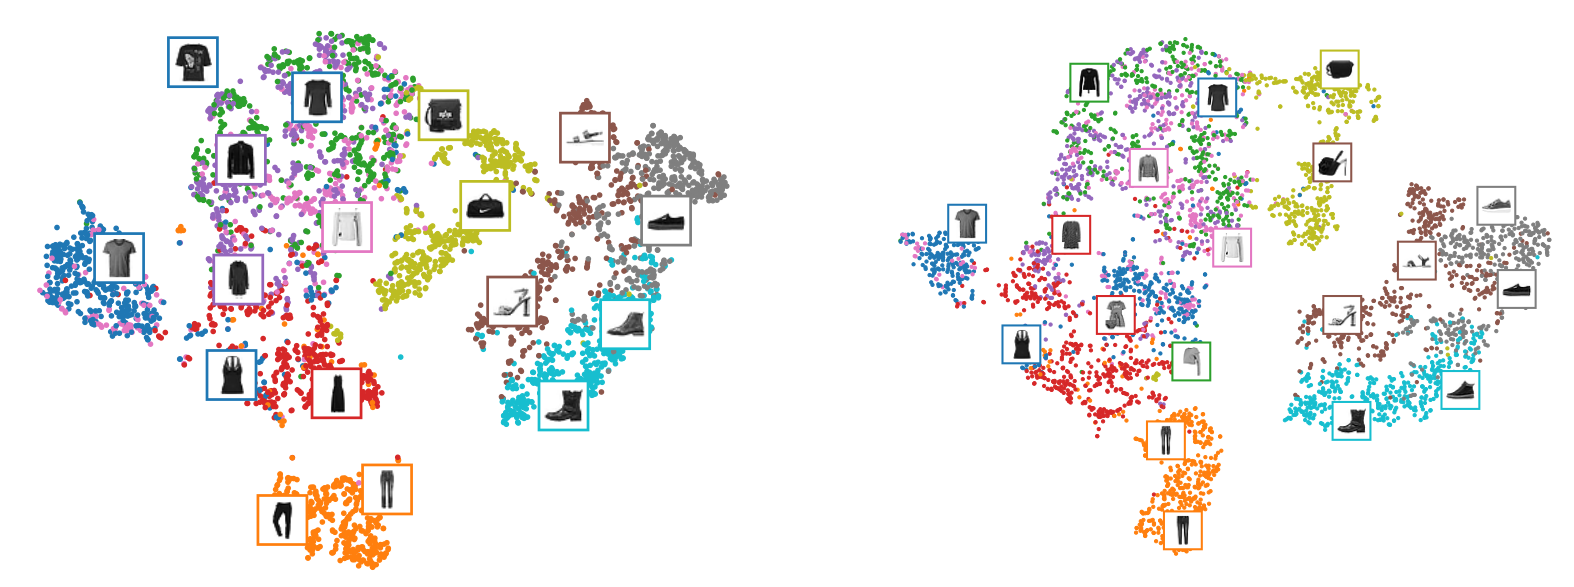
\includegraphics[width=\textwidth]{murphy_20_18.png} \\

\scriptsize Source: Murphy, Fig. 20.18 \normalsize
\end{center}
\caption{MNIST auto-encoder latent space points}
\label{fig:mnist_autoencoder_latent_space}
\end{figure}

Auto-encoders find applications for example in face recognition, feature detection, anomaly detection or data augmentation. The latter is achieved by generating novel output from points in the latent space that are close to the position of the original observation. That is, once the auto-encoder is trained, one encodes a given observation or image, adds a small amount of noise to the latent space vector, and then decodes into a new image. A similar use of auto-encoders is denoising, where images with noise are reconstructed by the decoder. After training the auto-encoder, a noisy input can be encoded into a latent space vector and the decoder then creates a noiseless output from that latent space vector. Figure~\ref{fig:murphy_20_19} shows two examples. In the left panel, Gaussian noise has been added to the input (top), the bottom row shows the denoised output. In the right panel, random pixels in the input have been dropped out, the bottom row shows the reconstructed images.

\begin{figure}
\begin{center}
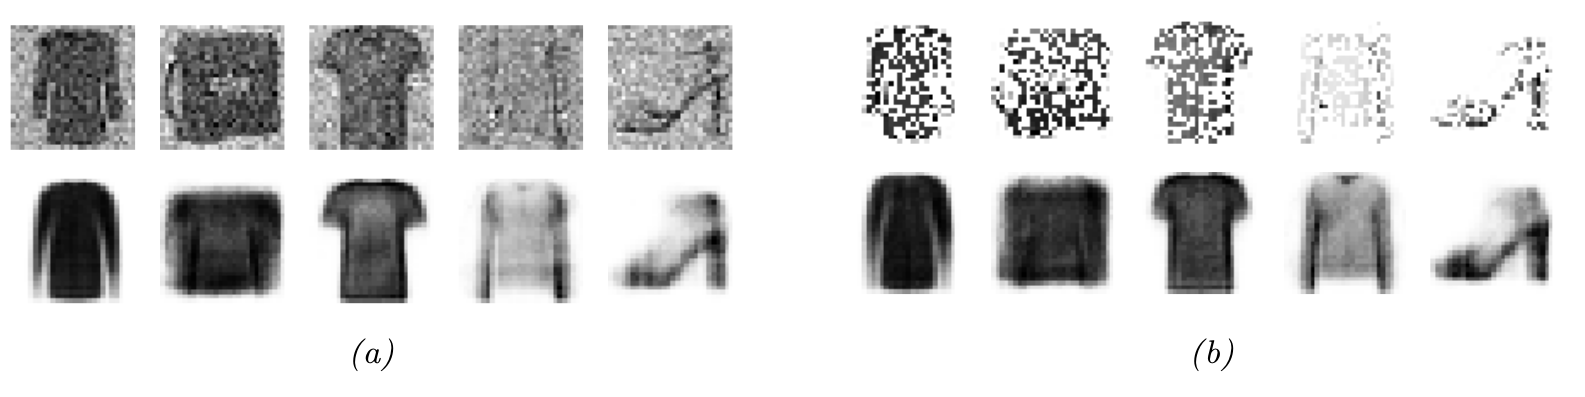
\includegraphics[width=\textwidth]{murphy_20_19.png} \\

\scriptsize Source: Murphy, Fig. 20.19 \normalsize
\end{center}
\caption{MNIST denoising auto-encoder}
\label{fig:murphy_20_19}
\end{figure}


\begin{resourcebox}
Complete implementations of the following auto-encoder examples are available on the following GitHub repo:

\url{https://github.com/jevermann/busi4720-ai} \\

The project can be cloned from this URL:

\url{https://github.com/jevermann/busi4720-ai.git}
\end{resourcebox}

The following Python code block shows a simple auto-encoder using TensorFlow. First, the encoder is defined as a sequence of fully-connected layers. It receives image data in multiple dimensions, flattens the dimensions before passing the data through a sequence of fully-connected layers, ending it with a final latent space output dimension of $30$. 

\begin{pythoncode}
from tensorflow.keras import layers
from tensorflow.keras import models
import keras

encoder = models.Sequential([
    layers.Flatten(),
    layers.Dense(1000),
    layers.Dropout(0.25),
    layers.Dense(500),
    layers.Dropout(0.25),
    layers.Dense(30)
])
\end{pythoncode}

The decoder is defined in the next Python code block. It takes as input a set of points in a latent space of $30$ dimensions. A sequence of fully-connected layers transform the latent space vector into a vector with $28 \times 28$ dimensions, which is reshaped into a two-dimensional image output. In this example, the decoder is the inverse of the encoder, that is, the types of layers are identical and their sequence is reversed. However, this is not necessary and the decoder can use an entirely different architecture than the encoder, as long as the final decoder output dimensions/shape matches the dimensions/shape of the encoder input.

\begin{pythoncode}
decoder = models.Sequential([
    layers.Dense(500),
    layers.Dense(1000),
    layers.Dense(28*28),
    layers.Reshape(target_shape=(28, 28))
])
\end{pythoncode}

Combining the encoder and the decoder in a sequential model yields the complete auto-encoder model:

\begin{pythoncode}
auto_encoder = models.Sequential([encoder, decoder])
\end{pythoncode}

The next code block loads the MNIST Fashion data set and transforms the image pixel values from integers to floating point numbers in the range $[0,1]$.

\begin{pythoncode}
(x_train, y_train), (x_test, y_test) = \
                    keras.datasets.fashion_mnist.load_data()
x_train = x_train / 255.0
x_test = x_test / 255.0
\end{pythoncode}

Finally, the auto-encoder model is compiled with MSE loss and trained on the data set:

\begin{pythoncode}
auto_encoder.compile(loss="mse")
auto_encoder.fit(x_train, x_train, 
                 epochs=5, validation_data=(x_test, x_test))
\end{pythoncode}

As a variation, the following two Python code blocks show a CNN architecture for both encoder and decoder. As noted above, it is not necessary that encoder and decoder have the same architecture, the same types or the same number of layers. For example, the fully-connected encoder can be connected to the CNN decoder below for a complete auto-encoder.

\begin{pythoncode}
encoder = models.Sequential([
    layers.Reshape([28, 28, 1], input_shape=[28, 28]),
    layers.Conv2D(16, (3, 3), padding="same", activation="relu"),
    layers.MaxPool2D((2, 2)),
    layers.Conv2D(32, (3, 3), padding="same", activation="relu"),
    layers.MaxPool2D((2, 2)),
    layers.Conv2D(64, (3, 3), padding="same", activation="relu"),
    layers.MaxPool2D((2, 2))])
\end{pythoncode}

\begin{pythoncode}
decoder = models.Sequential([
    layers.Conv2DTranspose(32, (3, 3), strides=2, 
               activation="relu", input_shape=[3, 3, 64]),
    layers.Conv2DTranspose(16, (3, 3), strides=2, 
               padding="same", activation="relu"),
    layers.Conv2DTranspose(1, (3, 3), strides=2, 
               padding="same", activation="sigmoid"),
    layers.Reshape([28, 28])])
\end{pythoncode}


\begin{infobox}
While the encoder and decoder in the examples here have the same architecture, this need not be the case! One could encode with a CNN and decode with a dense network, or any other combination of architectures.
\end{infobox}

\FloatBarrier

\section{Variational Auto-Encoders (VAE)}
\label{sec:vae}

Variational auto-encoders (VAEs)\index{VAE|see {Variational auto-encoder}}\index{Variational auto-encoder} take the idea of an auto-encoder one step further in that they add a probabilistic element. The main advantage is that VAEs can generate new images, not simply reconstruct or denoise images. The principle of a VAE is shown in Figure~\ref{fig:murphy_20_22}. While the auto-encoder above encodes the input into a point in a latent space, the VAE encodes the input into a probability distribution in the latent space, characterized by distributional parameters. In the example in Figure~\ref{fig:murphy_20_22} the distribution is a Gaussian with mean and variance vectors. The covariances between the latent space dimensions are assumed to be zero, that is, the latent space dimensions are assumed to be independent of each other. In practice, rather than using the variance (which is always positive), the log of the variance is used as this is in $(-\infty, +\infty)$.

The model can be re-parameterized\index{Reparameterization trick} so that instead of sampling from a Gaussian distribution with a mean and variance vector for decoding or generation, one can sample from a normal Gaussian distribution, shown in Figure~\ref{fig:murphy_20_23}. The left size shows the original parameterization of the model, whereas the right panel shows the re-parameterization. This re-parameterization is also useful for generative sampling, when constructing entirely new outputs as it allows sampling from a normal Gaussian that requires no knowledge of means and variances.

\begin{figure}
\centering
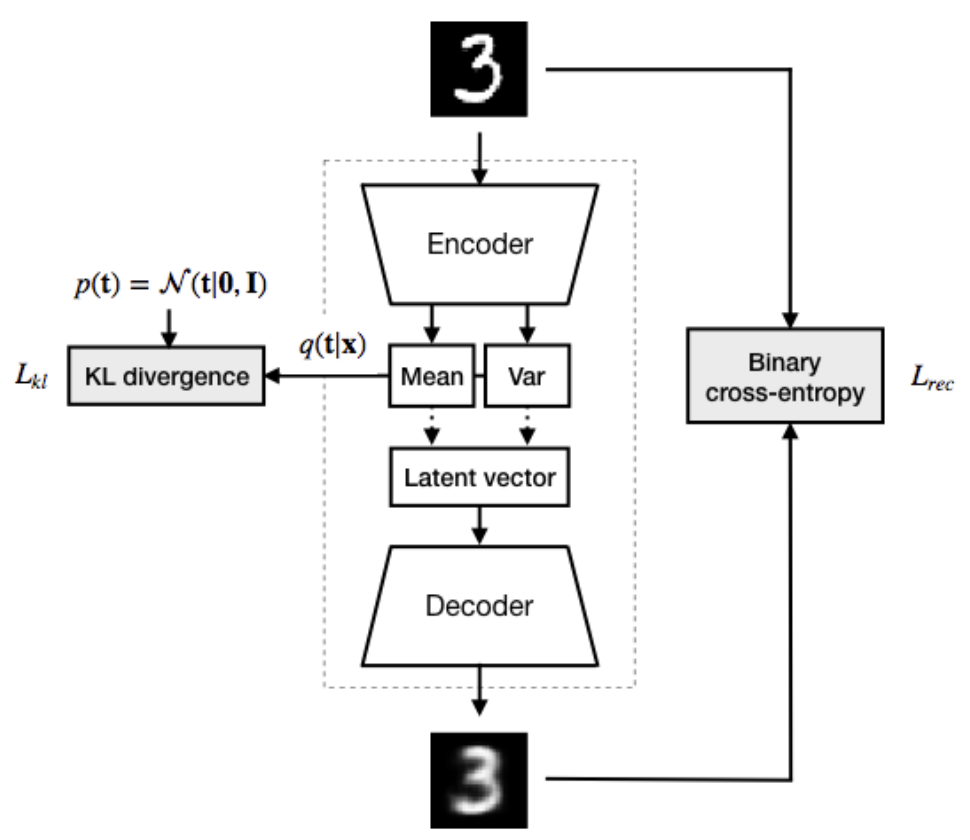
\includegraphics[height=2.5in]{murphy_20_22.png}\\

\scriptsize Source: Murphy, Fig. 20.22 \normalsize
\caption{Variational auto-encoder}
\label{fig:murphy_20_22}
\end{figure}


\begin{figure}
\begin{center}
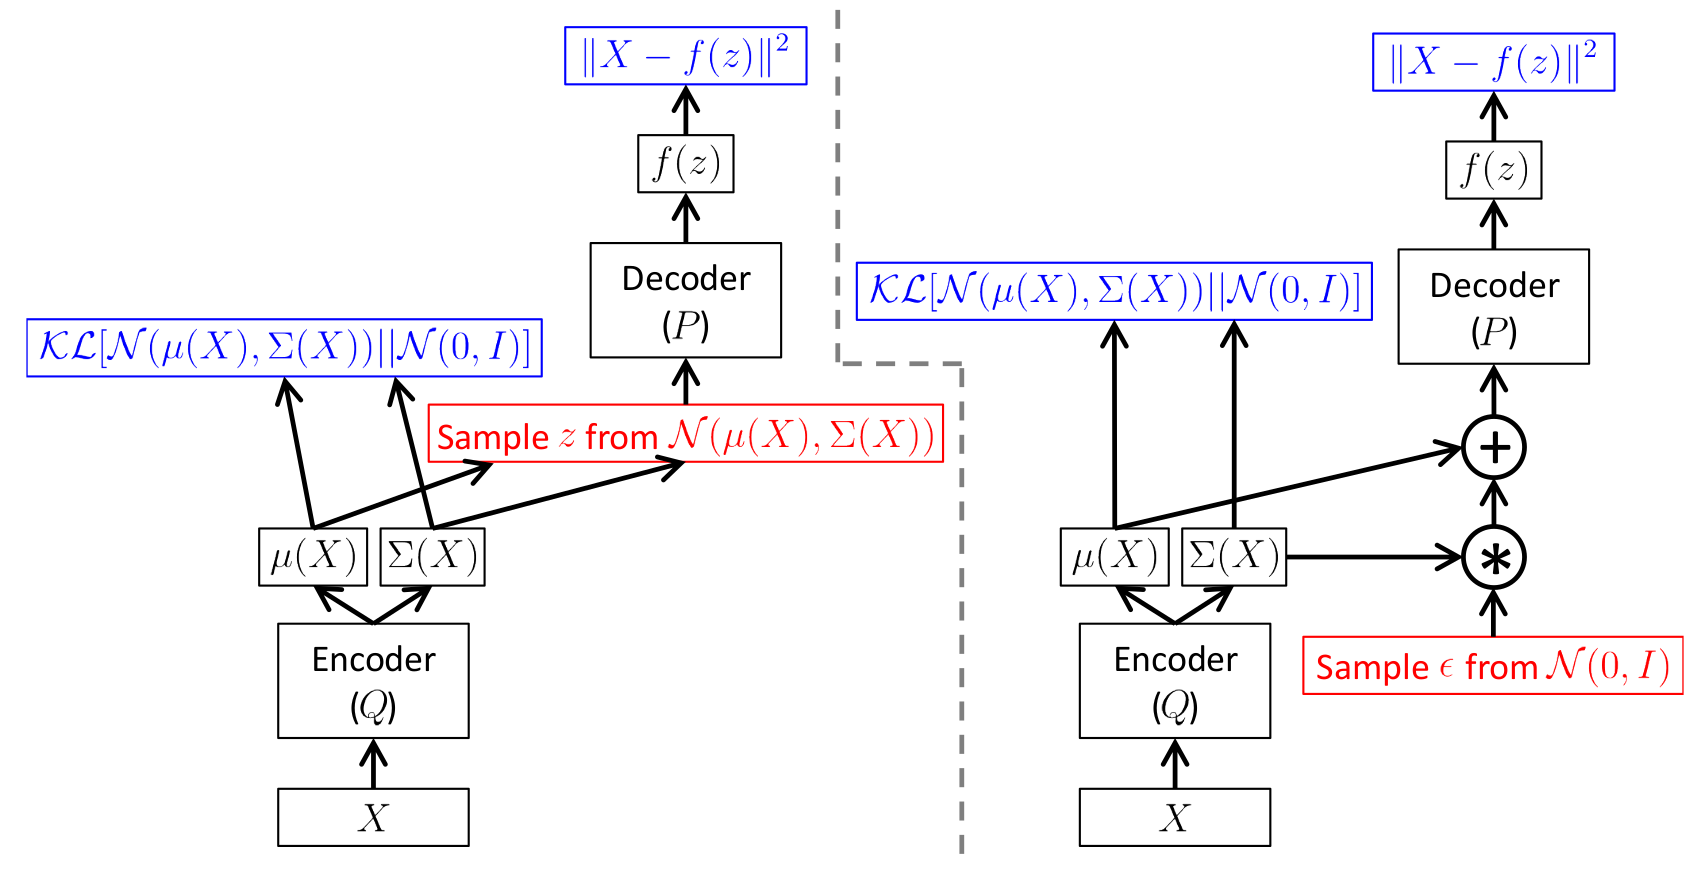
\includegraphics[width=\textwidth]{murphy_20_23.png}\\

\scriptsize Source: Murphy, Fig. 20.23 \normalsize
\end{center}
\caption{Variational auto-encoder re-parameterization}
\label{fig:murphy_20_23}
\end{figure}

VAEs generally outperform deterministic auto-encoders, as shown in Figure~\ref{fig:murphy_20_24} that compares VAEs (left panel) with deterministic auto-encoders (right panel) on an MNIST digits image reconstruction task (input at top, output at bottom). Both models can successfully reconstruct images. However, they perform very differently when generating novel output, shown in Figure~\ref{fig:murphy_20_25}. The deterministic auto-encoder (right panel) has never been trained on 'random' input, so is unable to decode a random sample from the latent space into sensible output. As shown in Figure~\ref{fig:mnist_autoencoder_latent_space}, there are large gaps between the areas into which images are mapped. Sampling from such gaps yields unrealistic output, as the decoder has not been trained on such input. In contrast, the VAE can generate realistic output from random input, as shown in the right panel. The representation as means and variances ensures that the latent space is continuous so that sampling a random point means the decoder knows how to decode this point. 

\begin{figure}
\begin{center}
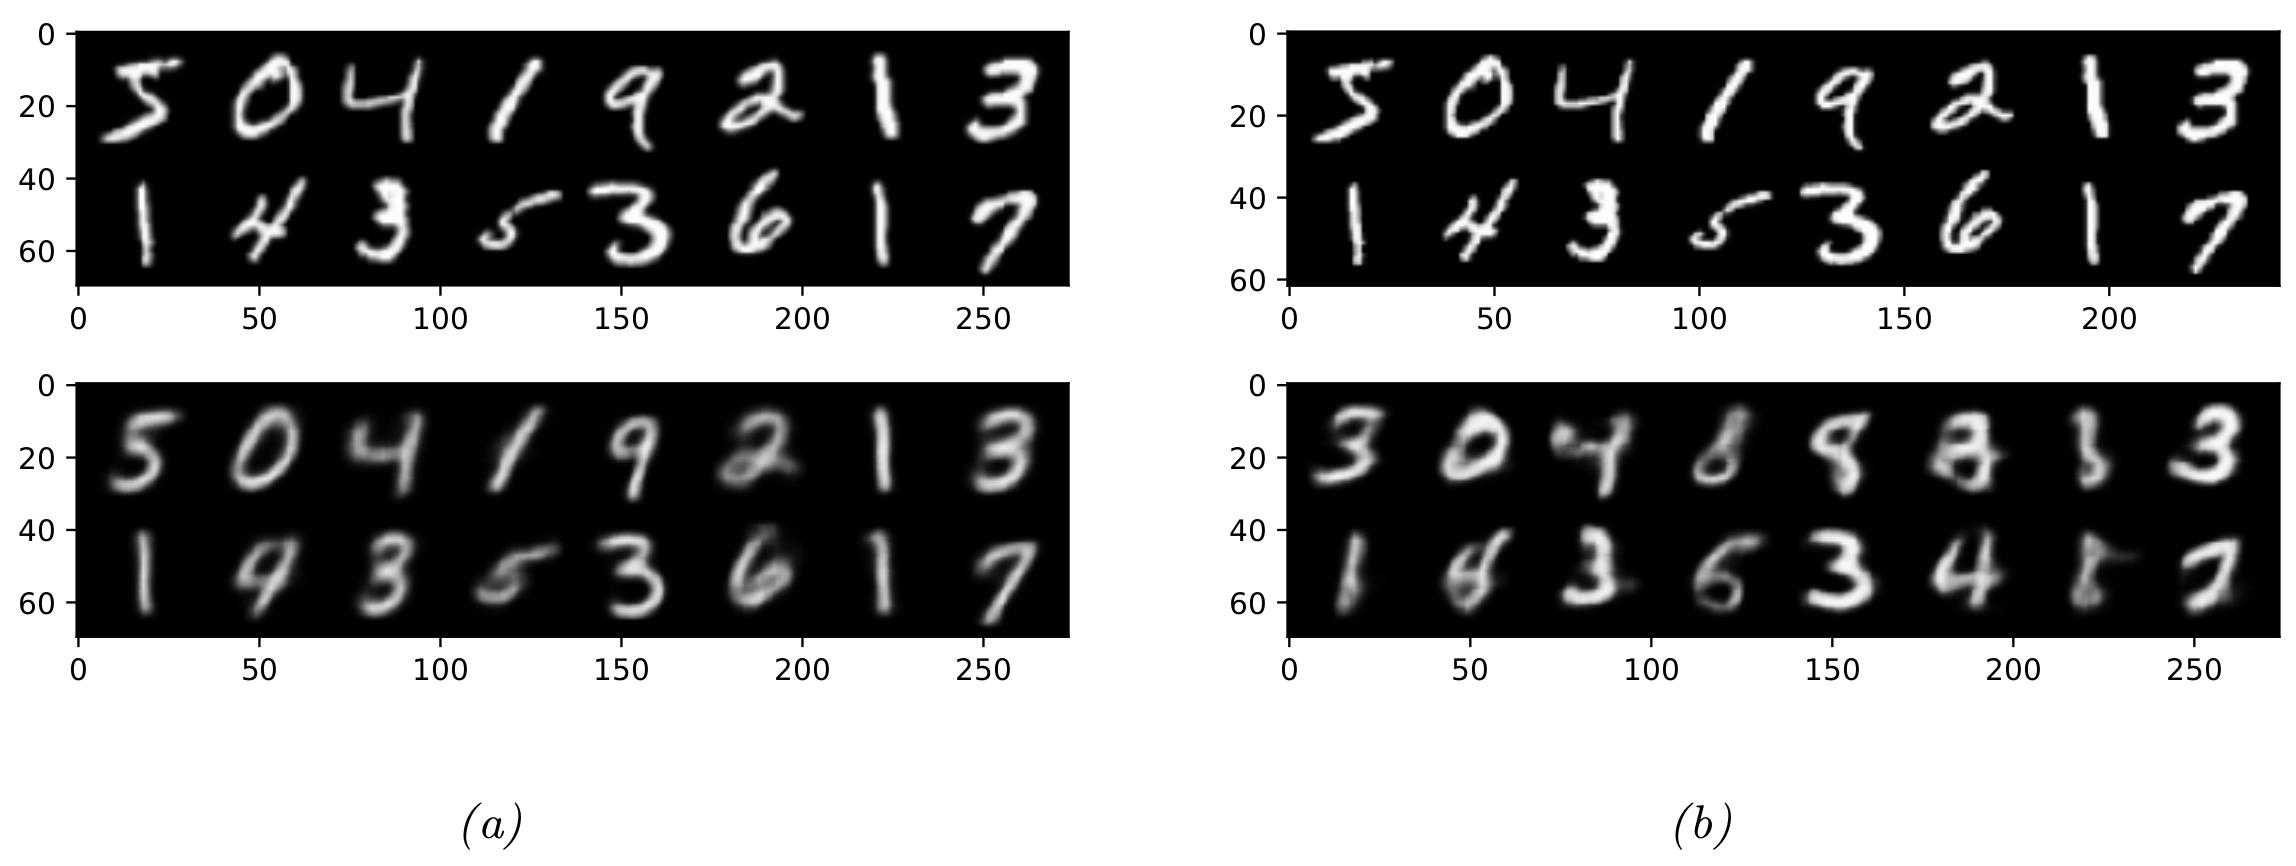
\includegraphics[width=\textwidth]{murphy_20_24.png}\\

\scriptsize Source: Murphy, Fig. 20.24 \normalsize
\end{center}
\caption{Comparison of VAE and AE on image reconstruction task}
\label{fig:murphy_20_24}
\end{figure}

\begin{figure}
\begin{center}
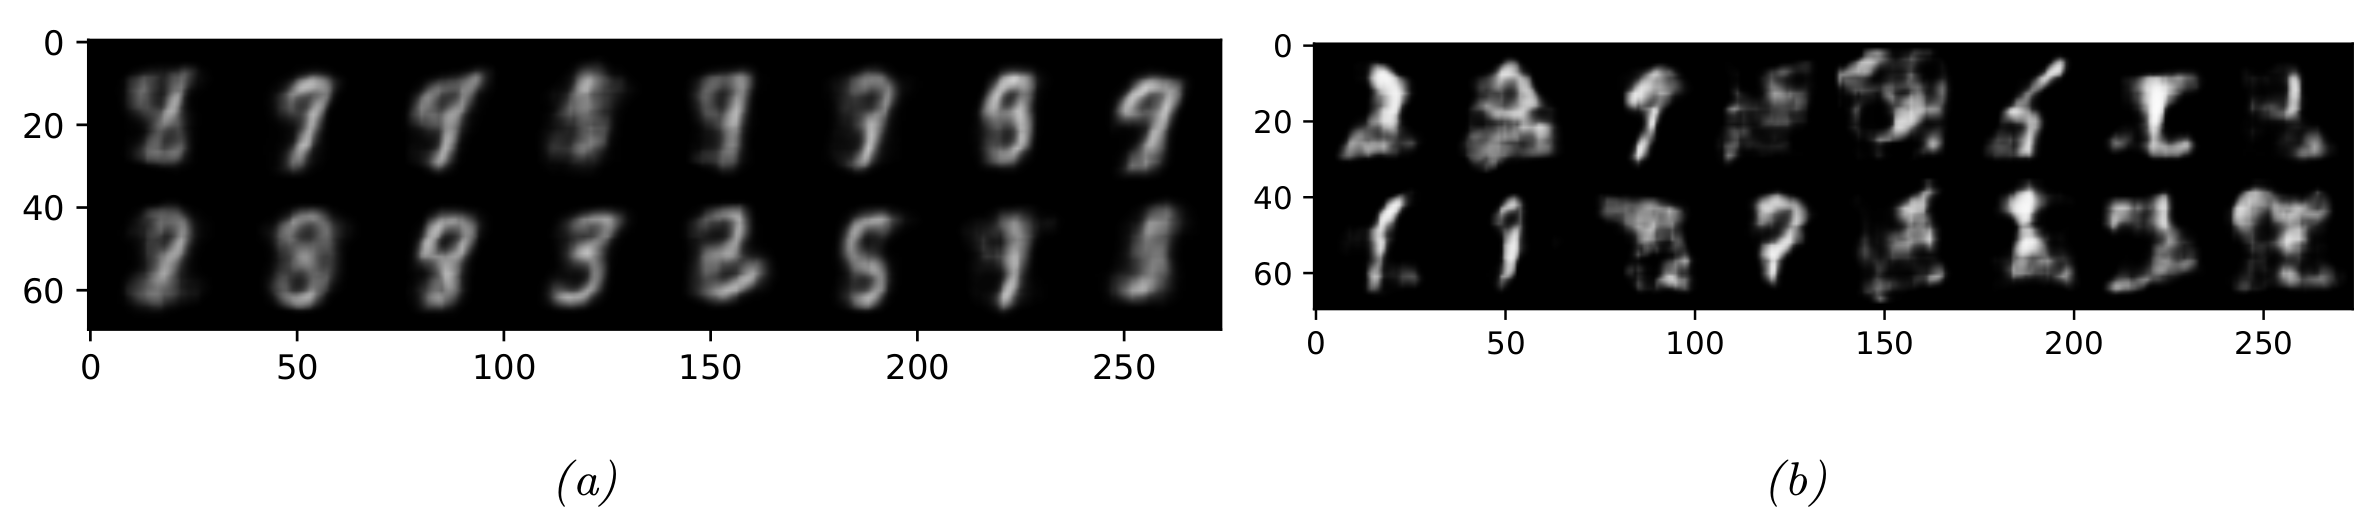
\includegraphics[width=\textwidth]{murphy_20_25.png}\\

\scriptsize Source: Murphy, Fig. 20.25 \normalsize
\end{center}
\caption{Comparison of VAE and AE on image generation task}
\label{fig:murphy_20_25}
\end{figure}

The following example shows how to implement a simple VAE in Python. It uses the same fashion MNIST data set as the auto-encoder example in the previous section and data loading and pre-processing is not shown here again. 

When defining a VAE in Python, the first step is to create a sampling layer\index{Sampling layers} that can be added after other neural network layers in the encoder. The following code block defines this as a type of Keras layer. Inputs to the layer are a vector of means and (log of) variances. The layer outputs a point in the latent space that is sampled from a normal distribution with those means and variances. Note that the layer actually samples from a normal Gaussian and the sampled point is then transformed by multiplying with the variance and adding the means, that is, using the re-parameterization described above and shown in Figure~\ref{fig:murphy_20_25}.

\begin{pythoncode}
import tensorflow as tf
import keras
from tensorflow.keras import layers

class Sampling(layers.Layer):
    def call(self, inputs):
        z_mean, z_log_var = inputs
        batch = tf.shape(z_mean)[0]
        dim = tf.shape(z_mean)[1]
        epsilon = tf.random.normal(shape=(batch, dim))
        return z_mean + tf.exp(0.5 * z_log_var) * epsilon
\end{pythoncode}

The encoder of a VAE\index{Encoder} in the following Python code block begins with a CNN whose output is flattened. The vector of 10 means and the vector of 10 log-variances are then created using a fully-connected layer (without activation function, that is, simply a matrix multiplication). That is, the latent space in this example has 10 dimensions. The sampling layer is added to take the means and log-variances and create a vector in the 10 dimensional latent space. Because both the means and log-variances are computed from the flattened CNN output, this is not a sequential model, so the definition looks slightly different than for the auto-encoder above.

\begin{pythoncode}
# This is NOT a sequential model
encoder_inputs = tf.keras.Input(shape=(28, 28, 1))
x = layers.Conv2D(32, (3,3), activation="relu", 
             strides=2, padding="same")(encoder_inputs)
x = layers.Conv2D(64, (3,3), activation="relu", 
             strides=2, padding="same")(x)
x = layers.Flatten()(x)
x = layers.Dense(16, activation="relu")(x)

# Vector of means
z_mean = layers.Dense(10, name="z_mean")(x)

# Vector of log variances
z_log_var = layers.Dense(10, name="z_log_var")(x)

# Point in latent space
z = Sampling()([z_mean, z_log_var])

encoder = keras.Model(encoder_inputs, [z_mean, z_log_var, z])
\end{pythoncode}

The VAE decoder\index{Decoder} is essentially the same as the decoder of an auto-encoder shown above. It takes as input a point in the 10-dimensional latent space, uses a fully-connected layer to increase the dimensionality, reshapes it into a two dimensional image format and applies a sequence of 2D convolutional transpose operations to it. The output of the decoder is an image with the same dimensions as the input images to the encoder.

\begin{pythoncode}
# Decoder
latent_inputs = keras.Input(shape=(10,))
x = layers.Dense(7 * 7 * 64, activation="relu")(latent_inputs)
x = layers.Reshape((7, 7, 64))(x)
x = layers.Conv2DTranspose(64, (3, 3), activation="relu", 
             strides=2, padding="same")(x)
x = layers.Conv2DTranspose(32, (3, 3), activation="relu", 
             strides=2, padding="same")(x)
decoder_outputs = layers.Conv2DTranspose(1, (3, 3), 
             activation="sigmoid", padding="same")(x)
decoder = keras.Model(latent_inputs, decoder_outputs)
\end{pythoncode}

As indicated in Figures~\ref{fig:murphy_20_22} and \ref{fig:murphy_20_23}, the VAE loss consists of both the ''reconstruction loss'', that is, the difference between input and output images, and the loss of the difference between the normal Gaussian and the Gaussian distribution with the given means and variances. The two losses are simply added (in contrast to Fig.~\ref{fig:murphy_20_22}, the following example uses the MSE for the reconstruction error, as did the auto-encoder example above). This combination of losses ensures the model tries to generate normally distributed points in the latent space as well as good reconstructions of the inputs.

\begin{pythoncode}
def vae_loss(encoder, decoder, data):
    z_mean, z_log_var, z = encoder(data)
    reconstruction = decoder(z)
    mse_loss = keras.losses.MeanSquaredError()
    reconstruction_loss = mse_loss(data, reconstruction)
    kl_loss = -0.5 * (1 +
                      z_log_var -
                      tf.square(z_mean) -
                      tf.exp(z_log_var))
    kl_loss = tf.reduce_mean(tf.reduce_sum(kl_loss,axis=1))
    total_loss = reconstruction_loss + kl_loss
    return total_loss
\end{pythoncode}

\begin{resourcebox}
Adapted from: 

\small\url{https://keras.io/examples/generative/vae/}\normalsize \\

Complete implementation available on the following GitHub repo:

\small\url{https://github.com/jevermann/busi4720-ai}\normalsize \\

The project can be cloned from this URL:

\small\url{https://github.com/jevermann/busi4720-ai.git}\normalsize
\end{resourcebox}


\FloatBarrier

\section{Generative Adversarial Networks (GAN)}

A generative adversarial network\index{GAN|see {Generative adversarial network}}\index{Generative adversarial network} consists of two networks that compete with each other, as shown in Figure~\ref{fig:gan}. The generator network\index{Generator} creates output from random input, that is, it creates observations (e.g. images) from random samples of a latent space. The discriminator network\index{Discriminator} receives a combination of real and fake (that is, generated from a random latent vector) inputs and must classify them as either real or fake. The generator is trained to ''beat'' the discriminator network in that is should create images the discriminator classifies as real. On the other hand, the discriminator is trained to best identify fake images. Thus, training improves both the generator and the discriminator's performance. The fully trained GAN can subsequently be used to create realistic observations from random input, that is, it is a generative model. Figure~\ref{fig:gancat} shows an example of an image generated by a GAN trained on animal images.

\begin{figure}
\begin{center}
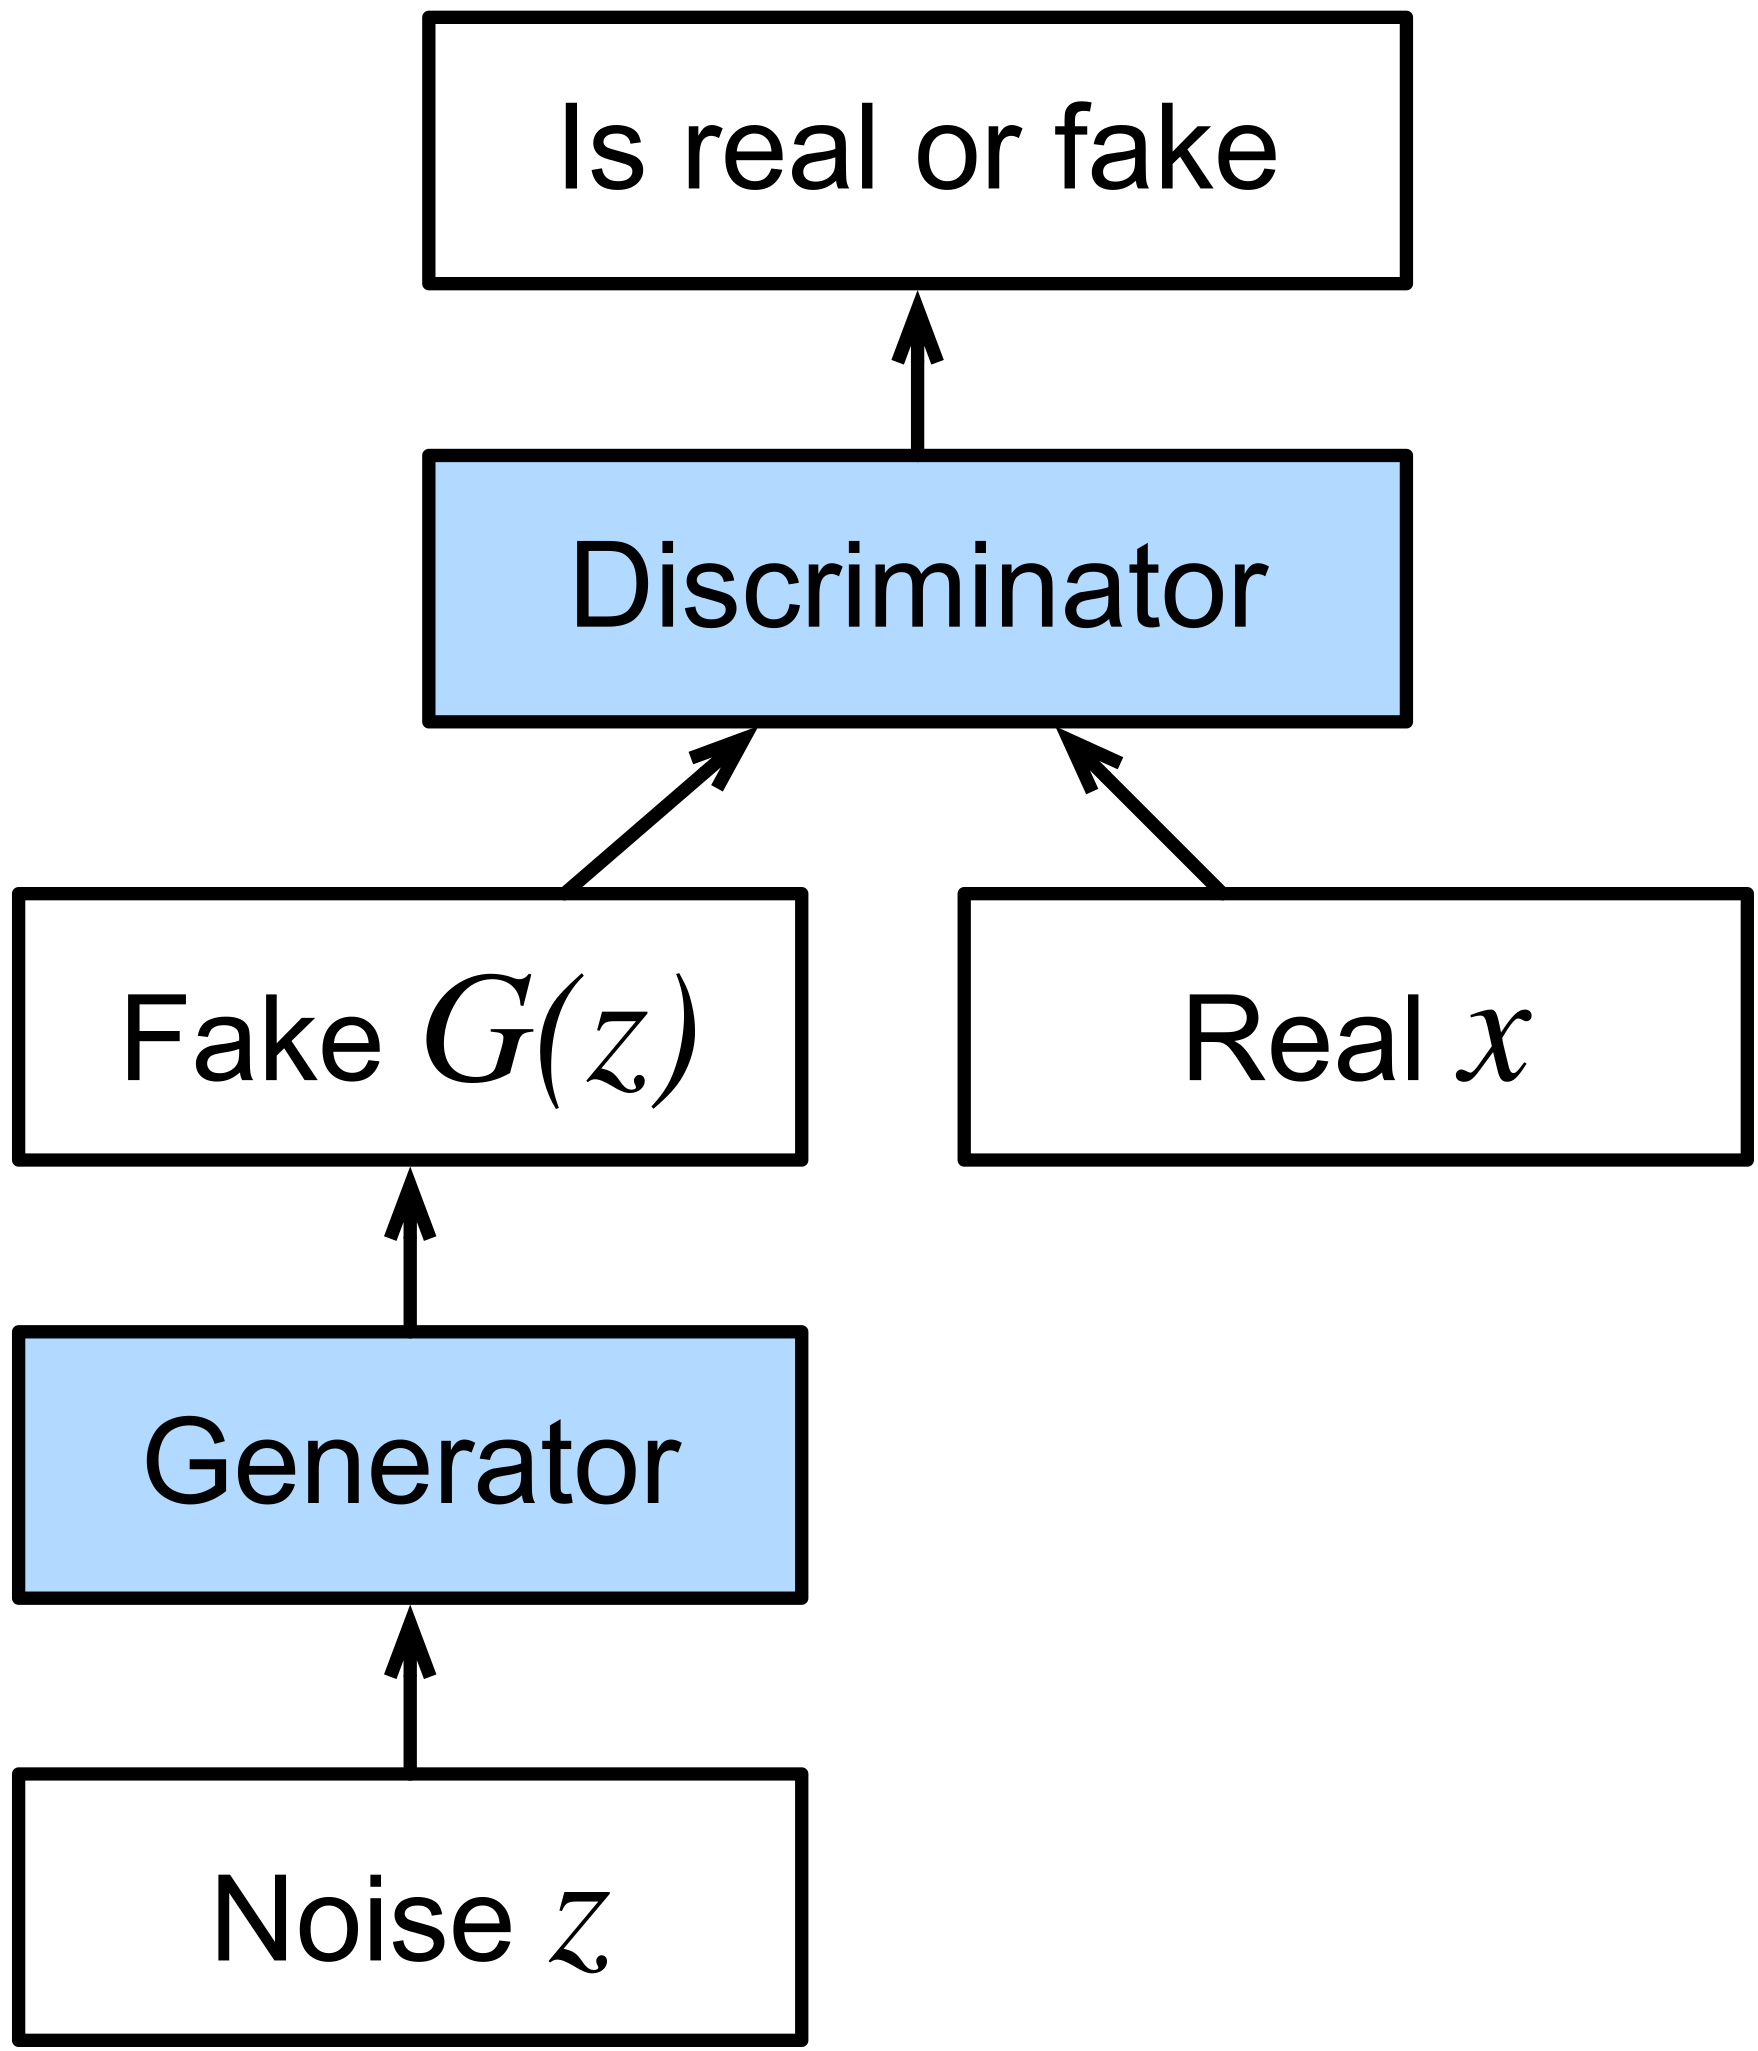
\includegraphics[height=2in]{Generative_adversarial_network.svg.png}\\

\scriptsize \url{https://commons.wikimedia.org/wiki/File:Generative_adversarial_network.svg} \normalsize
\end{center}
\caption{Generative adversarial network (GAN)}
\label{fig:gan}
\end{figure}

\begin{figure}
\begin{center}
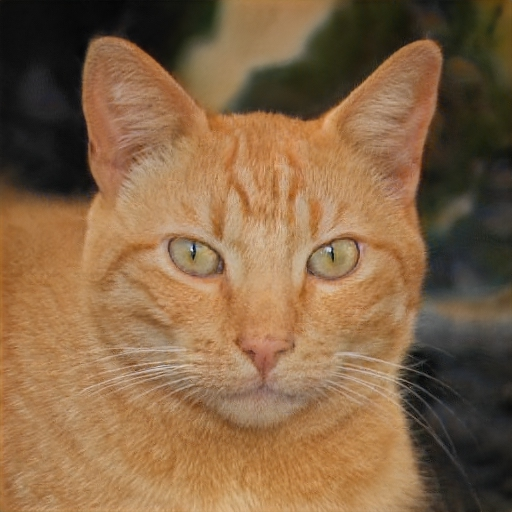
\includegraphics[height=2in]{GAN_Katze_StyleGAN2.png} \\

\scriptsize \url{https://commons.wikimedia.org/wiki/File:GAN_Katze_StyleGAN2.png} \normalsize
\end{center}
\caption{Image generated by a GAN}
\label{fig:gancat}
\end{figure}

In practice, a GAN implementation closely follows the principles shown in Figure~\ref{fig:gan}. The following Python example implements a simple GAN for generating images. It is based on the same fashion MNIST data set as the auto-encoder and VAE examples in the previous sections so that loading and pre-processing of the data set are not shown.

\begin{resourcebox}{GAN in Python}

Adapted from: 

\small\url{https://keras.io/examples/generative/dcgan_overriding_train_step/}\normalsize \\

Complete implementation available on the following GitHub repo:

\small\url{https://github.com/jevermann/busi4720-ai}\normalsize \\

The project can be cloned from this URL:

\small\url{https://github.com/jevermann/busi4720-ai.git}\normalsize
\end{resourcebox}

The discriminator of a GAN receives images to classify. It is implemented in the following Python code block as a CNN with the same structure as the encoder in the AE example earlier, except that the output is not a latent space vector but a single node that gives a probability for binary classification as either a real image or a fake image; hence the sigmoid activation function.

\begin{pythoncode}
discriminator = keras.Sequential([
    layers.Reshape([28, 28, 1], input_shape=[28, 28]),
    layers.Conv2D(16, (3, 3), 
        padding="same", activation="relu"),
    layers.MaxPool2D((2, 2)),
    layers.Conv2D(32, (3, 3), 
        padding="same", activation="relu"),
    layers.MaxPool2D((2, 2)),
    layers.Conv2D(64, (3, 3), 
        padding="same", activation="relu"),
    layers.MaxPool2D((2, 2)),
    layers.Flatten(),
    layers.Dropout(0.2),
    layers.Dense(1, activation="sigmoid")
])
discriminator.summary()
\end{pythoncode}

The generator of a GAN receives (random) latent space vectors to generate images from. In the following Python code block, the generator is implemented using the same CNN structure as the decoder in the AE example in the previous section.

\begin{pythoncode}
latent_dim = 10

generator = keras.Sequential([
    keras.Input(shape=(latent_dim,)),
    layers.Dense(3 * 3 * 10),
    layers.Reshape((3, 3, 10)),
    layers.Conv2DTranspose(32, (3, 3), strides=2, 
        padding="valid", activation="relu"),
    layers.Conv2DTranspose(16, (3, 3), strides=2, 
        padding="same", activation="relu"),
    layers.Conv2DTranspose(1, (3, 3), strides=2, 
        padding="same", activation="sigmoid"),
    layers.Reshape([28, 28])
])
generator.summary()
\end{pythoncode}

The training of a GAN on a single batch of real images involves training the generator, and subsequently training the discriminator. The following Python code block shows how the generator is trained. First, a set of \small\texttt{batch\_size}\normalsize random vectors of \small\texttt{latent\_dim}\normalsize dimensions in the latent space is created. These are passed to the generator to generate the ''fake'' images. The generated and real images are combined, as are the true class labels: A vector of ones for the generated images, and a vector of zeroes for the real images. 

\begin{pythoncode}
class GAN(keras.Model):
    def train_step(self, real_images):
        # Sample random points in the latent space
        batch_size = tf.shape(real_images)[0]
        rnd_latent_vectors \
            = tf.random.normal((batch_size, self.latent_dim))

        # Decode them to fake images
        gen_images = self.generator(rnd_latent_vectors)

        # Combine them with real images
        images = tf.concat([gen_images, real_images], axis=0)

        # Assemble labels discriminating real from fake images
        labels = tf.concat(
            [tf.ones((batch_sz, 1)), 
            tf.zeros((batch_sz, 1))], axis=0)
\end{pythoncode}

In the next Python code block, the set of images is passed to the discriminator which predicts whether an image is real or fake. The true labels and the discriminator predictions are then used to calculate the discriminator loss. The gradient of this loss is calculated with respect to the trainable parameters of the discriminator only, and is then used to update the trainable parameters of the discriminator.

\begin{pythoncode}
        # Train the discriminator
        with tf.GradientTape() as tape:
            predictions = self.discriminator(images)
            d_loss = self.loss_fn(labels, predictions)
            
        grads = tape.gradient(
            d_loss, 
            self.discriminator.trainable_weights)
        self.d_optimizer.apply_gradients(
            zip(grads, self.discriminator.trainable_weights))
\end{pythoncode}

In the next Python code block shows how the generator is trained. Another set of random latent space vectors is created, and a set of misleading labels (all zeros) is created. The latent space vectors are then passed to the generator and the generator output (a set of images) is passed to the discriminator for classification/prediction. The predictions are compared to the labels with the generator loss function, the generator loss gradient is computed, and the trainable parameters of the generator are updated.

\begin{pythoncode}
        # Sample random points in the latent space
        random_latent_vectors = \
            tf.random.normal((batch_size, self.latent_dim))

        # Assemble labels that say "all real images"
        misleading_labels = tf.zeros((batch_size, 1))

        # Train the generator 
        with tf.GradientTape() as tape:
            predictions = self.discriminator(
                self.generator(random_latent_vectors))
            g_loss = self.loss_fn(
                misleading_labels, predictions)

        grads = tape.gradient(
            g_loss, 
            self.generator.trainable_weights)
        self.g_optimizer.apply_gradients(
            zip(grads, self.generator.trainable_weights))
\end{pythoncode}

Because the generator and the discriminator are trained at the same time, their loss function does not necessarily decrease: A better generator will lead to a higher loss of the discriminator, and a better discriminator will lead to a higher loss of the generator. As both are improved, the losses need not decrease even though both aspects of the GAN improve. This makes monitoring the training of a GAN challenging. The following text block shows the output of a GAN training over 10 epochs:

\begin{textcode}
Epoch 1/10
1875/1875 [===] - 14s 7ms/step - d_loss: 0.0867 - g_loss: 4.3118
Epoch 2/10
1875/1875 [===] - 13s 7ms/step - d_loss: 0.1061 - g_loss: 3.9920
Epoch 3/10
1875/1875 [===] - 13s 7ms/step - d_loss: 0.1824 - g_loss: 2.8442
Epoch 4/10
1875/1875 [===] - 15s 8ms/step - d_loss: 0.2030 - g_loss: 2.5720
Epoch 5/10
1875/1875 [===] - 15s 8ms/step - d_loss: 0.2205 - g_loss: 2.4462
Epoch 6/10
1875/1875 [===] - 15s 8ms/step - d_loss: 0.2518 - g_loss: 2.2987
Epoch 7/10
1875/1875 [===] - 15s 8ms/step - d_loss: 0.2674 - g_loss: 2.2315
Epoch 8/10
1875/1875 [===] - 15s 8ms/step - d_loss: 0.2909 - g_loss: 2.1365
Epoch 9/10
1875/1875 [===] - 15s 8ms/step - d_loss: 0.2850 - g_loss: 2.1101
Epoch 10/10
1875/1875 [===] - 15s 8ms/step - d_loss: 0.2786 - g_loss: 2.1311
\end{textcode}

Other problems may occur when the discriminator becomes so good that it ''overpowers'' the generator. These issues can be addressed by reducing the learning rate for the discriminator, by reducing the number of CNN filters or removing entire CNN layers to make the discriminator less powerful, by adding noise to the labels when training the discriminator, or by adding more dropout layers or increasing the dropout rate in the discriminator. The inverse problem, that of the generator overpowering the discriminator can be addressed by making the discriminator more powerful using suggestions opposite the earlier ones for reducing the discriminator strength.

\FloatBarrier

\section{Review Questions}
\paragraph*{Data Augmentation}
\begin{enumerate}[nosep]
    \item What is the main difference between replicating training data and using data augmentation to increase training size? Why is one preferred over the other?

    \item Explain how data augmentation can act as a regularization technique in training deep learning models. Provide one example for image data and one for text data.

    \item Describe how data augmentation can help in class balancing. What issue does this address, and how does it affect the performance of a classifier?

    \item Give two examples of how data augmentation techniques can make training data more realistic. Why might overly ''clean'' or perfect data be a problem during training?

    \item What is SMOTE, and how does it generate new synthetic samples? What type of data is it best suited for? Illustrate your answer using the basic SMOTE procedure.

    \item Imagine a dataset for sentiment classification with very few negative reviews compared to positive ones. Suggest a complete data augmentation strategy involving techniques from the text, and justify how each method helps.
\end{enumerate}

\paragraph*{Transfer Learning \& Fine-tuning}

\begin{enumerate}[nosep,resume*]
    \item In your own words, explain the concept of transfer learning. What is the main assumption about the input data in transfer learning scenarios?

    \item Why would using a CNN trained on birds to classify cars not be a good example of transfer learning? What underlying principle does this violate?

    \item What are the two main phases of transfer learning? Briefly describe the purpose of each.

    \item What is the typical approach to fine-tuning in transfer learning for classification models? Which part of the model is usually replaced, and why?

    \item What are adapters in the context of transfer learning? How do they help address the risk of diverging too far from pre-trained parameter values?

    \item What is the purpose of initializing adapter parameters to zero, and how do skip-connections contribute to stable transfer learning?
\end{enumerate}

\paragraph*{Attention}

\begin{enumerate}[nosep,resume*]
    \item What is the purpose of the attention mechanism in neural networks, and how does it differ from traditional neural network processing of inputs?

    \item In the context of attention, explain the roles of the query ($Q$), key ($K$), and value ($V$) vectors. How are they used to compute the output?

    \item Why is attention particularly useful in sequence-to-sequence models for tasks like machine translation? What are some limitations of traditional encoder-decoder models that attention addresses?

    \item Define multi-headed attention and explain how it improves upon single-head attention. What are the main steps in computing multi-head attention?

    \item Describe self-attention and provide an example where it helps resolve ambiguity in a sentence. What makes self-attention different from the attention used between encoder and decoder?

    \item Compare and contrast the roles of attention scores, attention weights, and the final attention output. How are each computed and how do they contribute to the model's decision-making?
\end{enumerate}

\paragraph*{Transformers}

\begin{enumerate}[nosep,resume*]
    \item Why are Transformers able to process input sequences in parallel, unlike RNNs such as LSTMs and GRUs? What advantage does this provide during training?

    \item What are the two main pre-training tasks used in BERT? Briefly describe each and explain how they help the model learn language representations.

    \item How does BERT differ from ELMo in terms of model architecture? What type of neural network does each model use?

    \item Explain the components of BERT's input representation. What are the three types of embeddings used, and what does each represent?

    \item In ELMo, what is the purpose of using both forward and backward LSTM layers? How does this benefit the resulting word embeddings?
\end{enumerate}

\paragraph*{Auto-Encoders}
\begin{enumerate}[nosep,resume*]
   \item What are the main components of an auto-encoder, and what is its training objective? How does this differ from traditional supervised learning?

   \item In what ways can an auto-encoder be used for dimensionality reduction, and how is this similar to or different from Principal Component Analysis (PCA)?

   \item Why are auto-encoders generally not suitable as generative models? Refer to the structure of the latent space in your answer.

   \item What kinds of neural network layers can be used in the encoder and decoder of an auto-encoder? Is it necessary for both components to use the same architecture?
\end{enumerate}

\paragraph*{Variational Auto-Encoders (VAE)}
\begin{enumerate}[nosep,resume*]
   \item What is the main conceptual difference between a traditional auto-encoder and a variational auto-encoder (VAE) in terms of how input data is encoded into the latent space?

   \item Explain the structure of the latent space in a VAE. What do the vectors of means and variances represent, and why is it useful to assume independence among latent dimensions?

   \item Compare the generative capabilities of a deterministic auto-encoder and a VAE. Why is the VAE able to produce more realistic outputs when sampling random latent vectors?

   \item What are the two components of the total loss function in a VAE? Why is each component important for the model's performance?

   \item Explain how VAEs achieve continuity and coverage in latent space. How does this help prevent unrealistic or invalid outputs when generating new samples?
\end{enumerate}

\paragraph*{Generative Adversarial Networks (GAN)}

\begin{enumerate}[nosep,resume*]
   \item What are the two main components of a GAN, and what role does each play in the training process?

   \item How does the generator in a GAN learn to create realistic data? What is its training objective?

   \item What type of output does the discriminator produce, and what is its objective during GAN training?

   \item Why is GAN training considered adversarial? How do the generator and discriminator influence each other during training?

   \item Explain why GAN training can be challenging to monitor. What makes loss values difficult to interpret compared to standard models?

   \item Why is it important that the generator and discriminator are trained alternately rather than simultaneously on the same loss function?

   \item What are some signs that a GAN is not training properly? What could cause these issues, and how might they be addressed?
\end{enumerate}
